\documentclass[
% opciók nélkül: egyoldalas nyomtatás, elektronikus verzió
% twoside,     % kétoldalas nyomtatás
% tocnopagenum,% oldalszámozás a tartalomjegyzék után kezdődik
]{thesis-ekf}
\usepackage[T1]{fontenc}
\PassOptionsToPackage{defaults=hu-min}{magyar.ldf}
\usepackage[magyar]{babel}
\usepackage{mathtools,amssymb,amsthm}
\usepackage{xcolor,listingsutf8,caption}
\usepackage[final]{pdfpages}
\renewcommand{\lstlistingname}{kód}
\lstdefinestyle{user1}{
	inputencoding=utf8,
	basicstyle=\footnotesize,
	numbers=left,
	xleftmargin=2cm,
	xrightmargin=2cm,
	breaklines,
	backgroundcolor=\color{gray!20},
	frame=tblr,
	framesep=3pt,
	keywordstyle=\bfseries\color{blue},
	commentstyle=\itshape\color{teal},
	captionpos=b
}
\footnotestyle{rule=fourth}
\def\UrlBreaks{\do\/\do-}

\newtheorem{tetel}{Tétel}[chapter]
\theoremstyle{definition}
\newtheorem{definicio}[tetel]{Definíció}
\theoremstyle{remark}
\newtheorem{megjegyzes}[tetel]{Megjegyzés}

\begin{document}
	\institute{Matematikai és Informatikai Intézet}
	\title{Szakdolgozati konzultációk támogatása webes rendszerrel}
	\author{Vereczki Bálint Zoltán\\programtervező informatikus BSc}
	\supervisor{Balla Tamás\\tanársegéd}
	\city{Eger}
	\date{2021}
	\maketitle
	\tableofcontents
	
	\chapter*{Bevezetés}
	Életünkben egyre nagyobb területén van jelen az internet. Bárhol, bármikor hozzáférhetünk a zsebünkben hordott mobilkészülékünkről, pár érintés után elérhetjük a legfrissebb információkat és híreket. Terméket és ételt rendelünk, tájékozódunk, hivatalos ügyeket intézünk, kapcsolatot tartunk, zenét és filmet nézünk, mindezt a világhálón. Ezen tevékenységek révén egyre interaktívabb weboldalak készültek az évek során, melyek ki tudják szolgálni ezeket az igényeket.
	
	A felsőoktatásban elsődlegesen preferált kommunikációs forma a személyes konzultáción kívül az email. A legtöbb ügyintézés e-mail-es levelezéssel történik, ez pedig egyes esetekben problémákhoz vezethet. A rengeteg üzenet között előfordul, hogy egy-egy fontos üzenet elkerüli a figyelmet. A jelenlegi járványhelyzet akadályozza a személyes beszélgetés lehetőségét, így csupán az online kommunikációra hagyatkozhatunk.
	
	A szakdolgozatom célja ezen okoknál fogva egy olyan webes platform létrehozása, amely mind az oktatók, mind a hallgatók munkáját nagyban megkönnyíti és elősegíti a szakdolgozat elkészültének ideje alatt. Lehetőséget nyújt a hallgatók, szakdolgozatok, konzultációs időpontok menedzselésére, határidőre megadott feladatok kiírására és azokon keresztül való visszajelzésre.
	
	Szakdolgozatomban kitérek a webre, mint platformra és a webes alkalmazások mögött álló architektúrákra. Áttekintek néhány, a mai piaci trendek alapján leginkább használt keretrendszert, majd kiválasztom közülük azokat, amelyekkel az alkalmazásomat fogom elkészíteni. Ezt követően bemutatom a szoftver terveit és az elkészült alkalmazást.
	
	\chapter{Téma elméleti kifejtése}
	\section{A web, mint platform}
	Az egész világot behálózó számítógépes hálózatot internetnek nevezzük. Az internetre kapcsolódó számítógépek a TCP/IP (Transmission Control Procotol / Internet Protocol) segítségével képesek az egymással való kommunikációra. Minden egyes csatlakozott eszköz egy egyedi azonosítót kap, amelyet IP címnek nevezünk.
	A weboldalakat az IP címek helyett könnyebben megjegyezhető domain címek alapján látogatjuk meg (például \emph{www.google.com}), melyeket az internetre kapcsolódó speciális szerverek a DNS azaz névszerverek fordítanak le a hozzájuk tartozó IP címre.\cite{howthewebworks}
	
	A fent említett protokollokon kívül számos jelentős protokoll létezik, melyeket más célokra tudunk használni. Jelentősebb protokollok közül ilyenek például\cite{internetprotocols}:
	\begin{itemize}
		\item UDP (User Datagram Protocol)
		\item FTP (File Transfer Protocol)
		\item SSH (Secure Shell)
		\item \emph{HTTP} (Hypertext Transfer Protocol)
	\end{itemize}
	
	Az internet által használt TCP (Transmission Control Protocol) egy megbízható, kapcsolatorientált, végpont-végpont közötti kétirányú adatfolyamot biztosító protokoll. Megbízhatósága onnan ered, hogy az adatfolyam küldése közben nyugtázással biztosítja az adat megérkezését, hiba esetén pedig újrapróbálkozik az adat továbbításával.
	
	Az UDP protokoll úgynevezett datagram alapon szállítja az adatot. A datagramban tárolódik a forrásport, célport, adat hossza, az ellenőrzőösszeg és maga a küldeni kívánt adat. Ellentétben a TCP-vel, nem biztosítja az üzenet megérkezését, olyan esetekben optimális a használata, ahol nem feltétlenül szükséges a csomag megérkeztéről való visszaigazolás.
	
	Az FTP állományok számítógépek közötti átvitelére használatos protokoll, melynél két csatorna épül ki. Amikor a kliens csatlakozik az FTP szerverhez mindkét oldalon kiépül a vezérlő csatorna (Control Process), melyen keresztül a kliens parancsokat adhat a távoli gépnek. Amint állományátviteli kérést adunk ki, kiépül az adatcsatorna, amin keresztül az adatcsere folyamata zajlik.
	
	Az FTP protokoll autentikáció szempontjából nem tekinthető biztonságosnak, sem a TLS (Transport Layer Security), sem az SSL (Secure Sockets Layer) titkosítási protokollokat nem támogatja, a bejelentkezéshez használt felhasználónév és jelszó titkosítás nélkül kerül küldésre a klienstől a szerverig. Ezen probléma megoldásaként nyújt alternatívát az SSH (Secure Shell) protokoll, amely biztonságos kapcsolatot épít ki a helyi és távoli számítógép között, és állományátvitelen kívül használható a távoli gép kezelésére, parancsok kiadására. Az SFTP protokoll SSH-t használ a kapcsolat kiépítéséhez, így biztonságos kapcsolatot biztosít az állományátvitelhez. Az autentikáció történhet jelszóval, illetve egy úgynevezett nyilvános kulccsal is.\cite{sshprotocol}
	
	A HTTP protokoll segítségével képes kommunikálni a kliens (böngésző) és a szerver. Megbízható kapcsolatra van szükség, nem szabad üzenetvesztésnek történnie, ezért a kommunikációhoz TCP protokollt használ, amely kérés-válasz formájában történik. Ez a protokoll állapotmentes, ami azt jelenti, hogy a szerver nem emlékszik korábbi kérésekre, minden kérést egymástól függetlenül kezel.\cite{httpdocs}
	
	Minden kérés 3 részből áll össze: a kérés parancsából, ami tartalmazza a kérés metódusát, erőforrás útvonalát és a HTTP verzióját. Ezen kívül fejlécadatokat, mint például a Host, User-agent, Content-Type, és opcionálisan üzenetet tartalmaz. A válasz szintén 3 részre osztható: HTTP státusz kód, fejlécadatok és az üzenet.
	
	Többféle HTTP metódussal lehet kérést küldeni, adat letöltéshez például a GET, feltöltéshez a POST, frissítéshez a PUT vagy PATCH, törléshez pedig a DELETE használható.\cite{clientserver_overview}
	
	\section{Webes architektúrák}
	A webes alkalmazások tekintetében többféle módon is megtervezhetjük a mögöttes architektúrát.
	A HTTP kérés-válasz modellje miatt, legkézenfekvőbb a kliens-szerver architektúra (\ref{fig:kliens_szerver}.~ábra).
	
	\begin{figure}[!h]
		\centering
		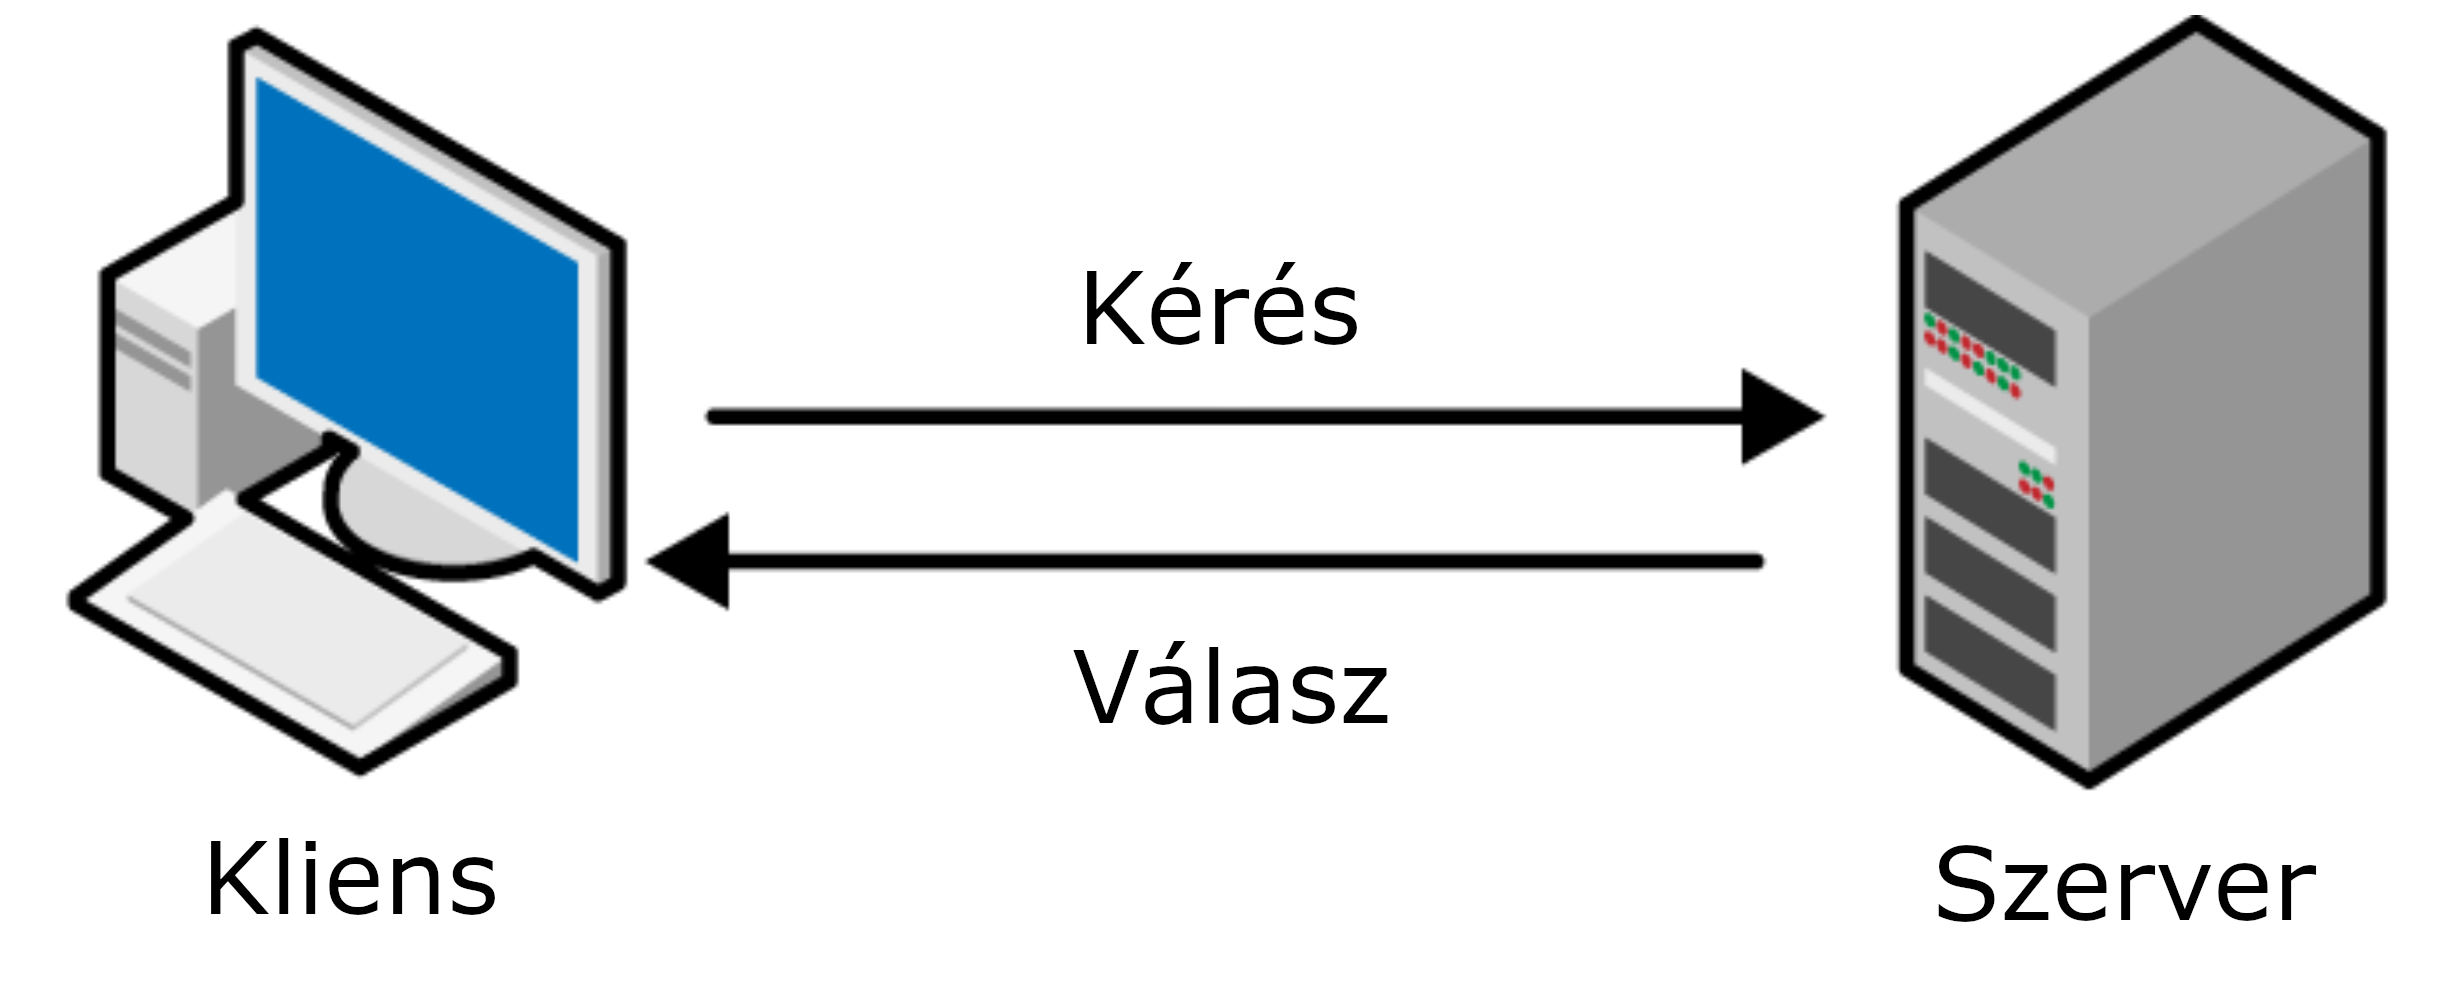
\includegraphics[width=6cm]{kepek/client_server_arch_magyaritva.png}
		\caption[A kliens-szerver architektúra]{A kliens-szerver architektúra\footnotemark}
		\label{fig:kliens_szerver}
	\end{figure}
	\footnotetext{Forrás: \url{https://madooei.github.io/cs421_sp20_homepage/assets/client-server-1.png}}
	
	A kliens-szerver architektúrának több fajtája létezik, az ezek közötti különbséget a rétegek száma határozza meg. Létezik kétrétegű (two-tier), háromrétegű (three-tier) architektúra, több réteg esetén pedig n rétegű (n-tier) architektúráról beszélhetünk.
	
	A kétrétegű architektúra résztvevői a kliens és a szerver. A kliens megjeleníti a felhasználói interfészt, majd az azon történt interakció után kérést küld a szervernek, és az onnan kapott választ feldolgozza és megjeleníti.
	A szerver passzív szerepet tölt be, várja a kliensek kéréseit, melyeket teljesít és visszaküldi nekik a választ.
	
	A fenti architektúrát egy újabb köztes réteggel bővítve háromrétegű (three-tier) architektúrát kapunk (\ref{fig:haromretegu}.~ábra).
	
	\begin{figure}[!h]
		\centering
		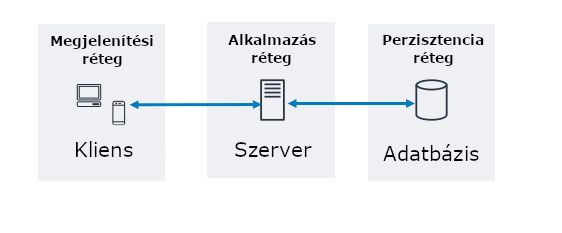
\includegraphics[width=12cm]{kepek/three-tier.png}
		\caption[A háromrétegű architektúra]{A háromrétegű architektúra\footnotemark}
		\label{fig:haromretegu}
	\end{figure}
	\footnotetext{Forrás: \url{https://docs.aws.amazon.com/whitepapers/latest/serverless-multi-tier-architectures-api-gateway-lambda/images/image2.png}}
	
	A háromrétegű architektúrában megkülönböztetjük a megjelenítési (presentation), alkalmazás (application), és perzisztencia (data) rétegeket.\cite{tierarchitecture}
	
	A megjelenítési réteg közvetlenül elérhető a felhasználó számára, mely a szervertől kapott adatoknak biztosít grafikus interfészt. Ehhez használatos a HTML leírónyelv, CSS stílusok és a JavaScript, amely segítségével dinamikussá és lényegesen interaktívabbá tehető a felület.
	
	Az alkalmazás rétegben található az összes szükséges üzleti logika, hidat alkotva a kliens és az adatbázis között. A kliensektől érkező kéréseket fogadja, kiértékel, logikai döntéseket hoz, adatokat validál és dolgoz fel, számolási feladatokat lát el, adatot továbbít a kérést indító kliens felé.
	
	Az adatbázis réteg feladata az adattárolás, és adathozzáférés biztosítása, melyet általában egy relációsadatbázis-kezelő rendszer (RDBMS) végez, mint például Oracle, MySQL, PostgreSQL. Relációs adatbázisszervereken kívül történhet NoSQL adatbázis-kezelő rendszeren is az adattárolás, ezek közül a legnépszerűbb megoldás a MongoDB.
	
	A kliens-szerver architektúra előnye, hogy nagyon könnyen skálázható újabb szerverek és kliensek beiktatásával, ezenfelül minden adat a szervereken tárolódik (centralizált adattárolás), így sokkal biztonságosabb is, mert szabályozható az egyes erőforrásokhoz való hozzáférés.
	
	Hátrányok közé sorolható, hogy gyakran eléggé drága szervereket kell vásárolni, illetve azok karbantartásához szakemberekre is szükség van.
	
	A legtöbb webalkalmazás a háromrétegű architektúrát alkalmazza, ugyanis sokkal könnyebb ezzel a munka. A rétegek egymástól függetlenül működnek, ezáltal ha valamin -- a rétegeket összekötő interfészeken kívül -- változtatás vagy frissítés történik, az nem érinti egyben az egész alkalmazást, csupán az adott réteget. Ezen kívül a fejlesztés szempontjából is sokkal könnyebb egy ilyen rendszeren dolgozni az elkülönített részegységek révén.
	% A rétegek egymástól függetlenül működnek, ezáltal ha valamin változtatás vagy frissítés történik az nem érinti egyben az egész alkalmazást, csupán az adott réteget. 
	
	\section{Webalkalmazáshoz alkalmazható technikák}
	Webalkalmazások készítésére számtalan programozási nyelv és keretrendszer elérhető a fejlesztők számára. Bizonyos időközönként (havonta / évente) több szervezet is (például Tiobe, StackOverflow\cite{stackoverflow_survey}, GitHub\cite{octoverse}) statisztikát készít fejlesztők által kitöltött kérdőívek, és adott kifejezésekre való keresések száma alapján az adott időszak legkedveltebb és legtöbbet használt programozási nyelveiről és keretrendszerekről.
	
	\begin{figure}[!ht]
		\centering
		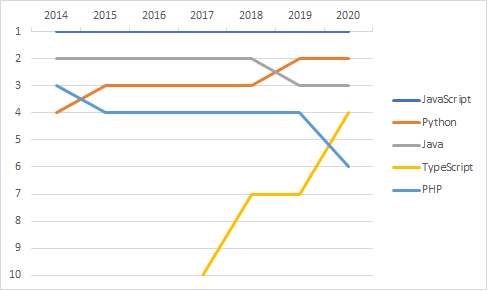
\includegraphics[width=9cm]{kepek/octoverse_languages_ranking.png}
		\caption{Programozási nyelvek ranglistája (2014-2020)}
		\label{fig:ranglista}
	\end{figure}
	
	A State of the Octoverse\cite{octoverse} a GitHub által minden évben elkészített felmérés, melyben a projektek és felhasználók adatait felhasználva készítenek statisztikát az előző évre vonatkozóan. Az fenti grafikonon néhány, a webes alkalmazásokhoz is használható nyelvet emeltem ki a 2014-től 2020-ig tartó időszakban.
	
	\Az{\ref{fig:ranglista}}.~ábra alapján egyértelműen látszik, hogy a JavaScript toronymagasan vezeti a ranglistát már 6 éve, míg a legtöbb weboldal által használt PHP népszerűsége az utóbbi időben csökkent. 2012-ben jelent meg a TypeScript, ami 2017-től kezdődően évről-évre népszerűbb a fejlesztők körében a statikus típusossága és objektumorientáltsága révén. Egyre nagyobb népszerűségnek örvend a Python is, habár elsődleges felhasználási területe nem a webfejlesztés, készült backendre alkalmazható keretrendszer.
	
	\chapter{Felhasznált technológiák ismertetése}
	\section{Kliensoldali technológiák}
	A 2006-ban megjelent jQuery\cite{jquery} könyvtár lehetőségek tárházát nyitotta meg a webfejlesztők felé. Segítségével rövidebb kóddal elérhető ugyanaz a működés, mint natív JavaScript esetén, és a különböző böngészők okozta kompatibilitási problémákra is megoldást nyújt. A könyvtárat a mai napig nagyon sok weboldal használja, ötvözve a fejlesztők által írt bővítményekkel pedig rengeteg problémára sokkal könnyebb megoldást találni, mint ha natív JavaScript-ben fejlesztene a programozó. Hátulütője, hogy sebességét tekintve jóval lassabb a JavaScript-nél és az SPA\footnote{Single Page Application} webalkalmazások idejében egyre elavultabbá válik, például a Bootstrap CSS keretrendszer esetében a legújabb, 5.~verzióban már kivezetésre került a könyvtár.
	
	\begin{figure}[!h]
		\centering
		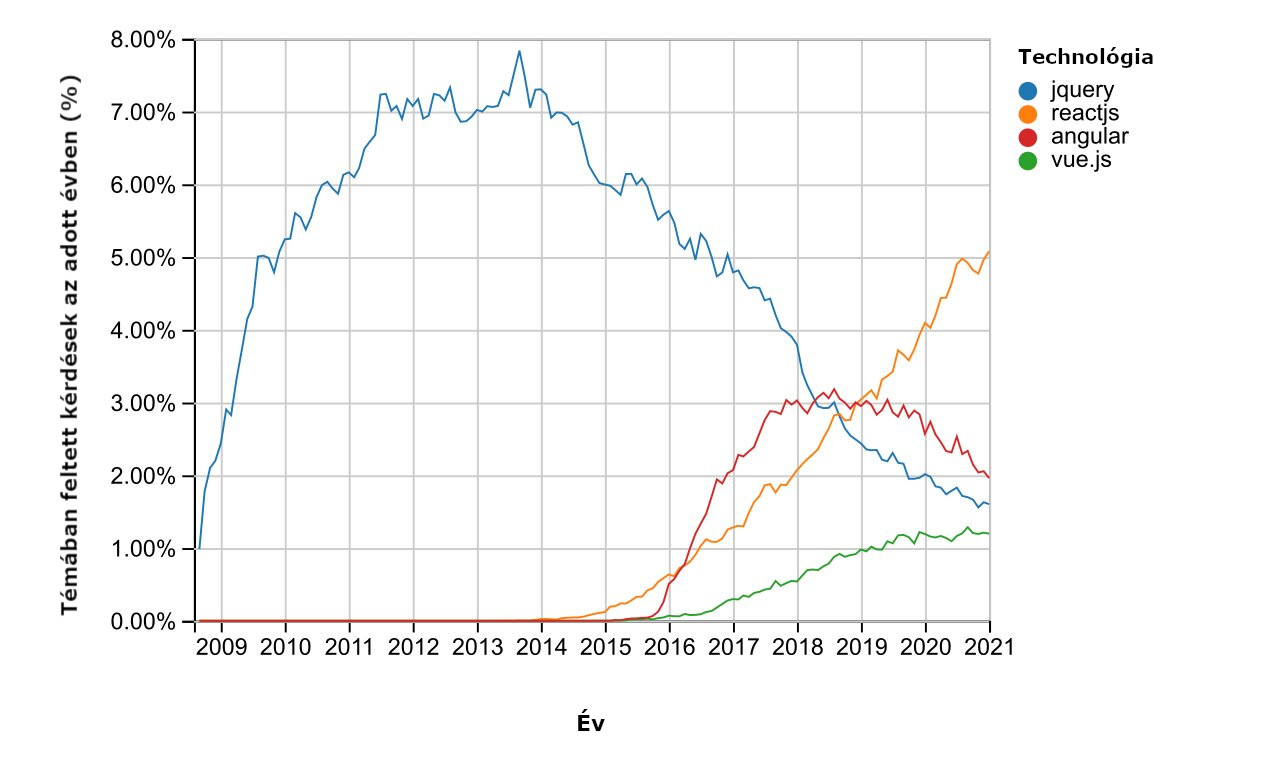
\includegraphics[width=11cm]{kepek/stackoverflow_js_trends_2021_magyar.jpg}
		\caption{JavaScript keretrendszerek népszerűsége\cite{stackoverflow_trends}}
		\label{fig:stackoverflow_trends}
	\end{figure}

	\Az{\ref{fig:stackoverflow_trends}}.~ábrán a Stackoverflow Trends adatai alapján készült grafikon látható, mely 2009-től 2021-ig bezárólag megmutatja, hogy egyes keretrendszerek mennyire népszerűek az oldalon feltett kérdések alapján. A piacot jelenleg 3 fő keretrendszer uralja, az Angular, a React és a Vue.js.
	
	\subsection[Angular]{Angular\cite{angulardocs}}
	Az Angular a Google által fejlesztett nyílt forráskódú keretrendszer, mely első kiadása 2016. szeptemberében jelent meg, az AngularJS második, továbbfejlesztett változataként. A keretrendszert TypeScript programozási nyelvben írták, és segítségével a HTML és TypeScript ötvözésével készíthetünk webalkalmazásokat, illetve natív mobilalkalmazásokat is.
	
	Egy Angular alapokon épülő webalkalmazás úgynevezett NgModule-okból áll, melyek komponensekből, szervizekből, és egyéb az adott modulhoz tartozó fájlokból állnak össze. A komponensek nézeteket tartalmaznak az adatok manipulálására és megjelenítésére, és service-ket használnak különféle specifikus feladatokra (például szerver oldal felé történő kérések küldésére).
	
	A view, azaz a nézet felelős az adatok megjelenítéséért. Ehhez az Angular-ban sablonokat (template) használhatunk, egy speciális Angular szintaxissal, amely kibővíti a HTML leírónyelvet, és több funkcionalitást biztosít, mint például a változók használata, eseménykezelés, és adatkötési technikák. Ezzel a szintaxissal definiált műveletek még a nézet megjelenítése előtt megváltoztatják a HTML elemeket, hogy azok már a kívánt adatokkal jelenjenek meg a böngészőben.
	
	Révén, hogy a sablonokban nem használhatunk JavaScript programkódot, az Angular úgynevezett beépített direktívákat használ péládul az iterációhoz (\emph{*ngFor}) és feltételvizsgálathoz (\emph{*ngIf}), de írhatunk saját direktívákat is.
	
	\lstinputlisting[style=user1,caption=*ngFor direktíva használata,label=kod-ngFor]{kodok/ngfor.txt}
	
	Service osztályokat azon adatoknak és programlogikának készíthetünk, melyek nem kifejezetten tartoznak egy nézethez, és a webalkalmazásunk akár több pontján is használni szeretnénk. Ezeket az osztályokat az \emph{@Injectable()} dekorátorral annotálva más osztályokban is felhasználhatjuk a függőség befecskendezés (dependency injection) segítségével.
	
	Az alkalmazásban történő útválasztás, átirányításokhoz a \emph{@angular/router} csomagot használhatjuk, mely automatikusan beépül a generált projektbe, ha a projektet a ,,\emph{ng new routing-app --routing}'' paranccsal generáljuk le az Angular CLI-n keresztül.
	
	Nagyobb alkalmazások esetén az alkalmazáson belüli állapotkezeléshez, az \emph{ngrx\footnote{\url{https://ngrx.io}}}, illetve \emph{ngxs\footnote{\url{https://ngxs.io}}} csomagokat használhatjuk, melyeket a React alkalmazásokhoz is használt Redux is nagyban inspirált.
	
	\subsection[React]{React\cite{vuecomparison}\cite{react}}\label{subs:react}
	A React a Facebook által fejlesztett, nyílt forráskódú keretrendszer, mely 2013 májusában jelent meg. Webes alkalmazásokon kívül használható platformfüggetlen mobilalkalmazások készítésére is a React Native keretrendszer segítségével.
	
	Webalkalmazásokban felhasználói interfész és azok komponenseinek készítésére alkalmazható. Ellentétben a többi keretrendszerrel, a program és megjelenítésért felelős logikát nem külön fájlokban, hanem egy komponensben központosítja. Ehhez a JSX\footnote{JavaScript XML}-et használhatjuk, ami egy JavaScript-et kibővítő szintaxis, mely a megjelenítéshez használatos HTML és egyéb komponens elemeken kívül JavaScript logikai programkódot is tartalmazhat.
	
	\lstinputlisting[style=user1,caption=JSX elem létrehozása,label=kod-jsx-elem]{kodok/react_jsx_elem.txt}
	
	Ezeket a komponenseket önállóan a böngésző nem tudja értelmezni, szükséges hozzá egy fordító is, a React a Babel JavaScript fordítót alkalmazza. A fordítás folyamán a JSX szintaxissal megírt kód minden egyes elemét átalakítja egy \emph{React.createElement()} metódushívássá, amely ellenőrzések sora után \az{\ref{kod-jsx-elem}}.~kódban látható JSX elemből \az{\ref{kod-jsx-object}}.~kódban látható JavaScript objektumot generálja le.
	
	\lstinputlisting[style=user1,caption=React.createElement() által generált objektum,label=kod-jsx-object]{kodok/react_jsx_object.txt}
	
	Ahhoz, hogy a létrehozott elemeket látni is lehessen a böngészőben, ki kell azokat rajzolni. A JavaScriptben a DOM\footnote{Document Object Model} segítségével lehet az oldal tartalmához hozzáférni, illetve azt módosítani. A DOM fa alapú hierarchiában tárolja az oldal felépítését, minden csomópontban egy-egy elemmel és annak tulajdonságaival. Amikor megváltoztatásra kerül egy elem a DOM-ban, akkor az egész oldalt újra kell rajzolni a hozzá tartozó stílusokkal együtt. Ennek hátránya, hogy nagyobb módosítások esetén túl sok időt vesz igénybe a DOM újrarajzolása. Ezen probléma megoldására fejlesztették ki a React DOM-ot.
	
	A React DOM a memóriában tárolja a felhasználói interfész másolatát, és biztosítja egy állapotváltozás esetén a szinkronizációt a DOM-mal. Folyamatosan vizsgálja az elemeket és azok gyerekelemeit, csupán akkor rajzolja őket újra, ha különböznek az előző állapotuktól, ezzel elkerülve az oldal teljes újrarajzolását.
	
	Az útválasztásra a React önmagában nem nyújt megoldást, ezt egy külső, a közösség által létrehozott és fejlesztett \emph{react-router} csomaggal valósíthatjuk meg. Nagyobb méretű alkalmazások esetén az alkalmazás állapotkezelésére több könyvtár, illetve architektúra is létezik. A legnépszerűbb megoldások közé tartozik a Flux\footnote{\url{https://facebook.github.io/flux/}}, amelyet a Facebook fejlesztett ki, a React közösség által fejlesztett Redux, illetve a MobX\footnote{\url{https://mobx.js.org/}}.
	
	\subsubsection[Redux]{Redux\cite{redux}}
	A Redux állapotkezelés alapelve, hogy az alkalmazás által használt adatokat egy központi helyen, a store-ban tároljuk. Az itt tárolt adatok önmagukban megváltoztathatatlan (immutable) objektumok.
	
	A store-ban tárolt adatok felülírásához folyamatokat (action) kell létrehoznunk (\ref{kod-action}.~kód). Minden folyamatnak meghatározott típusa van, ezen kívül szállíthat adatot is, amely a payload nevű mezőben található.
	
	\lstinputlisting[style=user1,caption=Részlet az authActions.js fájlból,label=kod-action]{kodok/code_action.txt}
	
	Az, hogy egyes folyamatok miként írják felül a store-ban tárolt értékeket a \emph{reducer} dönti el (\ref{kod-reducer}.~kód). Minden reducer rendelkezik egy initialState nevű objektummal, amely meghatározza az alapállapotot. Erről az objektumról készít másolatot a reducer, a megfelelő mezők módosításával, amely az új állapottá válik a storeban.
	
	\lstinputlisting[style=user1,caption=Részlet az authReducer.js fájlból,label=kod-reducer]{kodok/code_reducer.txt}
	
	Store készítéséhez (\ref{kod-store}.~kód) meg kell adnunk a használni kívánt reducer-eket, illetve megadhatunk opcionálisan kiegészítő funkciókat, mellyekkel nyomon követhetjük a folyamatokat, és a store-ban történő adatmódosulásokat. Ezek segítségével könnyebb a fejlesztés során a felmerülő hibák megkeresése és javítása.
	
	\lstinputlisting[style=user1,caption=Store létrehozása,label=kod-store]{kodok/code_store.txt}
	
	\subsection[Vue.js]{Vue.js\cite{vuecomparison}\cite{vuedocs}}
	A Vue.js nyílt forráskódú keretrendszer Evan You nevéhez köthető. A Google-nál Angular alapokon fejlesztett projekteket, majd az onnan való kilépését követően kezdte el fejleszteni a Vue.js-t, melyet a mai napig karbantart.
	
	A Vue akárcsak a React egy virtuális DOM-ot használ az állapotváltozások figyeléséhez, és a DOM-mal való szinkronizációhoz.
	
	A Vue által megjelenített oldalak az Angular keretrendszerben is használt sablonokkal kerülnek definiálásra. Ehhez egy HTML alapú sablon szintaxist használ, mely segítségével adatkötést végezhetünk. Szöveges adatkötés esetén a ,,Mustache'' szintaxist alkalmazhatjuk, azaz dupla kapcsos zárójelek közé kell a megjeleníteni kívánt adattagot tenni.
	
	A komponensekben a már Angular esetén is látott direktívák alkalmazhatóak iterációhoz, feltételvizsgálathoz, adatkötéshez. A Mustache szintaxis például elhagyható a \emph{v-html} direktíva használatával.
	
	\lstinputlisting[style=user1,caption=v-html direktíva használata,label=kod-v-html]{kodok/vue_v_html.txt}
	
	Számos más direktíva is elérhető, úgy mint a \emph{v-bind}, amely segítségével HTML attribútumokat tudunk adatkötéssel beállítani, a \emph{v-if} és a \emph{v-else} a feltételvizsgálathoz használható, a \emph{v-on:[esemenyNev]} direktívával pedig az eseményekhez köthetünk funkciókat. Ha a megjelenítés során iterációt szeretnénk használni, ahhoz a \emph{v-for} direktívát használhatjuk, amellyel tömbökön vagy egy objektum mezőin iterálhatunk végig.
	
	Az alkalmazásbeli útválasztáshoz elérhető egy, a keretrendszer által is támogatott könyvtár a \emph{vue-router}, mellyel kulcs-érték párokkal megadhatjuk, hogy egyes útvonalak esetén melyik komponensünket szeretnénk megjeleníteni.
	
	Az alkalmazáson belüli állapotkezelésre több könyvtár is elérhető, többek között a React ihlette Flux-hoz nem csak névben, de működésében is hasonló \emph{vuex\footnote{\url{https://vuex.vuejs.org/}}}.
	
	\section{Szerveroldali technológiák}
	\subsection[Express]{Express\cite{expressnodeintro}\cite{expressdocs}}
	A 2009-ben megjelent nyílt forráskódú, platformfüggetlen NodeJS által szerveroldalon is tudunk JavaScript nyelven írt programokat futtatni. A Google által fejlesztett V8 JavaScript motort használja, amely mellett egy alacsony-szintű I/O interfészt biztosít. A NodeJS telepítésekor megkapjuk az NPM\footnote{Node Package Manager} csomagkezelőt is, mellyel számtalan könyvtárat telepíthetünk az alkalmazásunkhoz.
	
	Ilyen könyvtár az Express is, ami egy viszonylag minimalista webes keretrendszer. Önmagában az Express az útvonalkezelés mellett alkalmas szerver oldalról történő kliens renderelésre és különböző sablonokat (például Pug, EJS) is támogat. Az útvonalakhoz a kérés-válasz ciklus között különböző funkciókat (middleware) rendelhetünk, amelyek hozzáférnek mind a kérés, mind a válasz objektumhoz. Ezeket a middleware-ket egész alkalmazásra, vagy egy-egy útvonalra vonatkozóan is alkalmazhatjuk, illetve hibakezelést, autentikációs ellenőrzést is megvalósíthatunk velük. 
	
	A keretrendszer tudását további NPM csomagok telepítésével tudjuk bővíteni. Számos könyvtár elérhető az NPM csomagkezelővel, melyekkel a sütiket (\emph{cookie-parser}), munkameneteket (\emph{cookie-session}), feltölteni kívánt fájlok kezelését (\emph{multer}) is elvégezhetjük.

	\lstinputlisting[style=user1,caption=Express szerver létrehozása,label=kod-express-alap-server]{kodok/express_server_alap.txt}
	
	Egy Express szerver létrehozásához (\ref{kod-express-alap-server}.~kód) inicializálnunk kell a projektet az \emph{npm init} parancs segítségével, majd telepíteni kell az Express csomagot az \emph{npm install express} paranccsal. A feltelepített csomagokat (másnéven modulok) a \emph{require()} metódus segítségével importálhatjuk különböző fájlokban.
	
	Az app nevű változó értékének adott \emph{express()} függvényhívás inicializál egy Express alkalmazást. Ezen a változón keresztül konfigurálhatjuk az útválasztást, a middleware funkciókat, és további beállításokat végezhetünk.
	
	Az útválasztáshoz a HTTP metódusoknak megfelelő nevű metódusokat használhatjuk (get, post, put, delete), melynek első paraméterként meg kell adnunk az elérési utat, majd második paraméterben egy úgynevezett callback metódust kell megadnunk, amely három paraméterrel rendelkezik:
	\begin{itemize}
		\item req: tartalmazza a HTTP kérést, paramétereket, üzenetet
		\item res: a HTTP választ reprezentálja, amelyet az Express a kérésre válaszul visszaküld
		\item next: meghívásával átadjuk az irányítást a soron következő middleware-nek
	\end{itemize}
	
	Lévén, hogy az Express egy minimalista keretrendszer, csak az alapvető eszközöket biztosítja, nincsen egy előre felépített struktúra, melyre építkezve egy jól karbantartható és fejleszthető alkalmazást készíthetünk. Erre nyújt megoldást a NestJS.
	
	\subsection[NestJS]{NestJS\cite{nestdocs}}\label{subs:nest}
	A nyílt forráskódú NestJS keretrendszer az egyik legfeltörekvőbb TypeScript backend keretrendszer jelenleg, mely ötvözi az objektumorientált és funkcionális programozás elemeit. Az Express szerveroldali webes alkalmazások estén nincsen egy előre definiált architektúra, amelyre építhetjük az alkalmazásunkat, a NestJS erre fókuszál: jól skálázható és jól struktúrált szerveroldali alkalmazások írására fejlesztették ki.  Fejlődését nagy mértékben befolyásolták a már megemlített frontend keretrendszerek, a React, Vue, de legnagyobb mértékben az Angular.
	
	Projekt generálásához a keretrendszer által nyújtott Nest CLI\footnote{Parancssoros felhasználói felület}-t kell feltelepíteni \emph{npm i -g @nestjs/cli} paranccsal, majd a ,,\emph{nest new projekt\_nev}'' parancssal tudunk projektet létrehozni.

	\begin{figure}[!h]
		\centering
		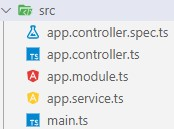
\includegraphics{kepek/nest_structure_light_jpg.jpg}
		\caption{Nest projekt struktúrája}
	\end{figure}
	
	A Nest alkalmazások úgynevezett modulokból, más néven feature-ökből állnak. Az alkalmazás gyökérmodulja az \emph{app.module.ts}, amely magába foglalja az alkalmazás összes többi modulját. Egy-egy modul több osztállyal kerül legenerálásra: saját kontroller osztállyal és az ahhoz tartozó egységteszt fájllal, saját service osztállyal és a modult egybeszervező module osztállyal. TypeScript keretrendszer révén a projektben több helyen is kötelező a dekorátorok használata, úgy mint modul, kontroller és service osztály létrehozása esetén is.
	
	Minden modul osztályt kötelező a \emph{@Module()} dekorátorral annotálni (\ref{kod-nest-module}.~kód). Modul generálásához a ,,\emph{nest g module modul\_nev}'' parancsot használhatjuk. Ebben az osztályban importálhatunk más modulokat, exportálhatunk az adott modulból a service-k közül azokat, amelyeket más modulban is el akarunk érni, illetve megadhatjuk az adott modul által használt kontroller és service osztályokat. A kontrollerek és service-k között megadott osztályokból automatikusan létrejön egy-egy példány, amelyet az objektumorientált programozásban használatos függőség befecskendezés technika segítségével használhatunk fel.
	
	\lstinputlisting[style=user1,caption=Module osztály tartalma,label=kod-nest-module]{kodok/nest_module.txt}
	
	A ,,\emph{nest g controller controller\_nev}'' parancs segítségével generálhatunk egy új kontrollert. Ezeket az osztályokat a \emph{@Controller()} dekorátorral kell annotálni, melyet felparaméterezve megadhatjuk az útvonal előtagját (prefix). Az osztály metódusait a HTTP kérés metódusainak megfelelő dekorátorokkal kell ellátni (@Get(), @Post(), @Put, @Delete()), innen tudja a keretrendszer, hogy az adott végpontot milyen metódussal lehet elérni. Ezeket a dekorátorokat paraméterezve megadhatjuk a végpontot. (\ref{kod-nest-controller}.~kód).
	
	\lstinputlisting[style=user1,caption=Kontroller osztály tartalma,label=kod-nest-controller]{kodok/nest_controller.txt}
	
	Új service-t létrehozni a ,,\emph{nest g service service\_nev}'' paranccsal tudunk (\ref{kod-nest-service}.~kód). Ezeket az osztályokat a \emph{@Injectable()} dekorátorral kell annotálni. Ez a dekorátor metaadatokkal látja el az osztályt, amely által az osztályt a keretrendszer IoC\footnote{Inversion of Control} konténere kezelni tudja. Az IoC konténer teszi lehetővé az automatikus függőség befecskendezést.

	\lstinputlisting[style=user1,caption=Service osztály tartalma,label=kod-nest-service]{kodok/nest_service.txt}
	
	Ahhoz, hogy a kontroller osztályban használni tudjuk a service metódusait injektálni kell azt a kontrollerbe a konstruktor paraméterei között (\ref{kod-nest-controller-di}.~kód).
	
	\lstinputlisting[style=user1,caption=Kontroller függőség befecskendezés,label=kod-nest-controller-di]{kodok/nest_controller_di.txt}
	
	Az alkalmazásban történő hibák kezeléséhez készíthetünk filtereket, melyeket a kontrollerekhez kapcsolhatunk a \emph{@UseFilters()} dekorátorral. Ezzel a megoldással kikerülhetjük azt, hogy minden kontroller metódus törzsében try-catch blokkba kelljen helyezni a service hívását, ugyanis a kontroller globálisan kezeli, ha egy, a filterben a \emph{@Catch()} dekorátorban definiált kivétel keletkezik.
	\newpage
	
	\lstinputlisting[style=user1,caption=MongoDB ObjectId cast hibát kezelő filter,label=kod-nest-exception-filter]{kodok/casterror_filter.txt}
	
	A NestJS alkalmazásokhoz készíthetünk úgynevezett Guard osztályokat is. Ezek a CanActive interfészt implementáló osztályok mindegyike egyetlen felelősséggel rendelkezik: eldöntik, hogy egyes kérések teljesítésre kerüljenek vagy sem. Felhasználásuk leginkább az autorizáció és a jogosultság alapú autentikációban merül ki.
	
	Láthatóan a NestJS számtalan eszközt biztosít az alkalmazások fejlesztéséhez külön könyvtárak használata nélkül is, stabil struktúrát biztosít webalkalmazások készítéséhez, melyet később könnyedén bővíteni lehet.
	
	\section{Adatbázis-kezelő rendszerek}
	A webalkalmazások egyik legfontosabb rétege az adatbázis, ahol az alkalmazás által felhasznált adatok kerülnek tárolásra. Többféle megoldást is alkalmazhatunk, webalkalmazásonként eltérő, hogy egyes esetekben milyen rendszert érdemes alkalmazni. A mai adatbázisrendszerek közül megkülönböztetjük a relációs és nemrelációs, másnéven NoSQL rendszereket. A két rendszer merőben eltér egymástól, mindkettőnek megvan a maga előnye és hátránya, illetve az a felhasználási területe, ahol optimálisabb és kényelmesebb a használata.
	
	\subsection[A relációs adatbázisok]{A relációs adatbázisok\cite{relationalvsnon-relational}\cite{ibm_sqlvsnosql}}
	A relációs adatbázisok (RDBMS) táblákban tárolják a logikailag összetartozó adatokat. A táblák sorokból és oszlopokból állnak, egy-egy sort rekordnak, míg egy oszlopot attribútumnak nevezünk.
	
	Működését tekintve abban tér el a NoSQL adatbázisoktól, hogy a táblákban különböző megszorításokat (például elsődleges vagy idegen kulcs), illetve tárolt eljárásokat definiálhatunk. A kulcsok által definiált kapcsolatokkal a lekérdezések során több táblából gyűjthetjük össze a kívánt adatokat. A megszorításokkal definiált táblák előnye, hogy biztosítják a táblákban az adatok integritását és konzisztenciáját, megelőzik az adatok helytelen módon történő frissítését, illetve törlését. Az integritást ezen felül az ACID séma biztosítja, mely az \emph{Atomitás}, \emph{Konzisztencia}, \emph{Izoláció} és \emph{Tartósság} szavak kezdőbetűiből áll össze.
	
	Az adatok lekérdezéséhez az SQL\footnote{Structured Query Language} lekérdezőnyelvet használhatjuk, mely kifejezetten a relációs adatbázisokhoz lett tervezve. Segítségével képesek vagyunk többek között az adatok lekérdezésére, felvitelére, frissítésére és törlésére.
	
	Az adatok mennyiségének növekedése révén fontos szempont a rendszer skálázhatóság, mely a relációs adatbázisok esetében felfelé, másnéven vertikálisan kivitelezhető. A vertikális skálázás során a számítási teljesítmény növeléséhez új vagy több processzorral, több memóriával, illetve gyorsabb háttértárral bővíthetjük a kiszolgálót.
	
	Legnépszerűbb relációs adatbázis rendszerek közé tartozik az SQL Server, MySQL, PostreSQL, Oracle.
	
	\subsection[A NoSQL adatbázisok]{A NoSQL adatbázisok\cite{mongo_typeofnosqldbs}\cite{aws_graphdb}}
	A NoSQL adatbázisok felépítése nagyban különbözik a relációs adatbázisok felépítésétől. Az adatok nem táblákban tárolódnak, és nincs lehetőség elsődleges vagy idegen kulcs megszorítások létrehozására sem. Olyan alkalmazások készítése esetén, melyekhez nem szükséges a relációs adatbázisok által nyújtott merev struktúra a NoSQL rendszerek nyújthatnak megoldást.
	
	A nemrelációs adatbázisok alapvetően az írás/olvasás műveletekre vannak kihegyezve, a sebességkülönbség a relációs adatbázisokkal szemben az azokban használt műveletek elhagyása révén érhető el (például táblák összekapcsolása). Adattárolási módjuk alapján több csoportot is megkülönböztethetünk, ezek közül a négy legnépszerűbb a dokumentumtárolók, az oszlop-orientált, a kulcs-érték pár, és a gráfadatbázisok.
	
	A dokumentumtárolók (például \emph{MongoDB}) többféle formátumban is tárolhatják a dokumentumokat, ezek közül a leggyakoribb a JSON, BSON\footnote{Binary JSON}, illetve XML\cite{mongodb_json_bson}. JSON esetében alapvetően csupán szövegek, számok, logikai értékek és tömbök tárolhatóak, a BSON ezen támogatott típusok kibővítésében segít, általa dátumokat és nyers bináris adatokat is tudunk tárolni, illetve a bináris felépítés által gyorsabb feldolgozási időt biztosít. Lehetőségünk van a dokumentumok egymásba ágyazására, így a lekérdezéskor azokat együtt megkapjuk, nincs szükség az adatok összegyűjtésére, mint az SQL esetén, ezzel is meggyorsítva az adatlekérést. Ezenfelül flexibilis struktúrát biztosít, ha idővel változnának az alkalmazás igényei, akkor annak igénye szerint egyszerűen és könnyen módosítható az adatbázis felépítése.
	
	A relációs adatbázisok soronként tárolják a rekordokat, ezzel szemben léteznek oszlop-orientált NoSQL rendszerek amelyek analitikai szempontból kínálnak gyors megoldást (például \emph{Cassandra}). Az alapötletük az, hogy a lekérdezések során csak abból az oszlopból kerülnek lekérdezésre az adatok, amelyekre egy-egy számítás során szükségünk van, így a számítás szempontjából szükségtelen adatok ignorálásra kerülnek.
	
	A NoSQL rendszerek legegyszerűbb megvalósítása a kulcs-érték párokat tároló adatbázisok (például \emph{Redis}), ahol egy-egy attribútumhoz (kulcs) egy-egy értéket párosítunk.
	
	Habár a NoSQL jelentése a nem-SQL vagy nemrelációs adatbázis, a gráfadatbázisokban (például \emph{OrientDB}) fontos az adatok közötti kapcsolat. Minden adat egy csúcsban tárolódik, melyek közötti kapcsolatot az őket összekötő él jelöli. Minden élt két csúcspontja (kiindulási és vég), típusa és iránya írja le. Az ilyen módon tárolt adatokat a kapcsolatok révén könnyen bejárhatjuk, nincs szükség a relációs adatbázisokban használt táblakapcsolásokra.
	
	\section{Összegzés}
	Ebben a fejezetben összehasonlítottam a legnépszerűbb technológiákat a kliens, a szerver és adatbázis szempontjából.
	A webalkalmazást a MERN (MongoDB -- Express -- React -- NodeJS) stack-ben helyet foglaló technológiákkal fogom megvalósítani.
	
	A React által használt JSX szintaxis rengeteg lehetőséget rejt magában a különböző újrafelhasználható komponensek készítéséhez, az alkalmazás állapotkezeléséhez pedig a jól dokumentált, számos kiegészítővel rendelkező Redux-ot használhatjuk.
	
	Szerveroldalon a NestJS keretrendszer mellett döntöttem az általa kínált eszközök, paradigmák és a TypeScript programozási nyelv támogatása miatt.
	
	A MongoDB egyszerű, flexibilis, remek eszköztárral rendelkezik a dokumentumok kezeléséhez, a dokumentumok egybeágyazásának lehetősége pedig praktikus megoldás a kliensoldali program számára.
	
	\chapter{Specifikáció}\label{chp:specifikacio}
	\section{Feladatspecifikáció}
	Egy olyan webalkalmazás készítését tűztem ki célul, amely elősegíti a szakdolgozatok elkészülésének ideje alatt mind az oktatók, mind a hallgatók munkáját és hatékonyabbá teszi a kommunikációt, illetve az elvégzendő feladatok nyomonkövetését.
	
	\subsection{Felhasználói szerepkörök}
	Az alkalmazás felhasználóit jogosultságaik alapján három szerepkörre lehet felosztani: ügyintéző, oktató és hallgató.
	A felhasználók kizárólag a szerepkörük által elérhető funkciókhoz és adatokhoz férnek hozzá. Minden felhasználó képes jelszavát megváltoztatni, illetve saját adatlapját megtekinteni.
	
	
	\subsubsection{Ügyintézők}
	\begin{figure}[!h]
		\centering
		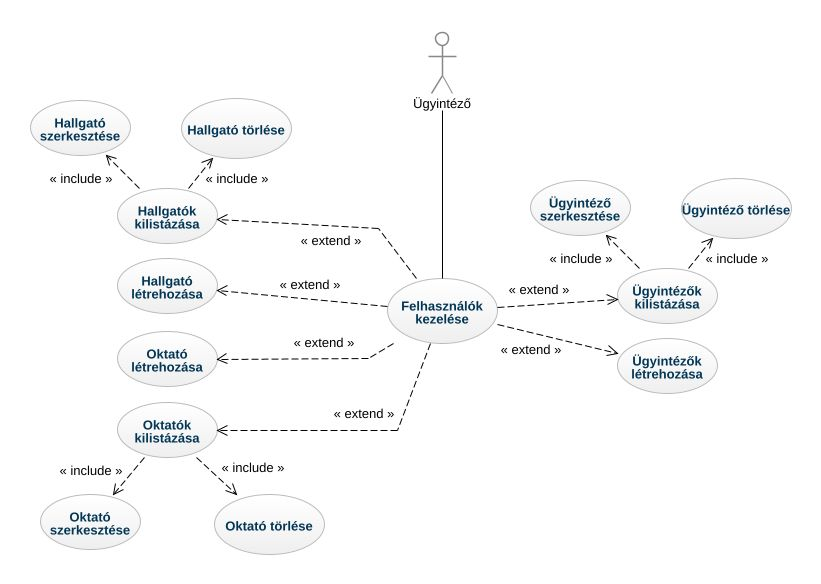
\includegraphics[width=14cm]{kepek/admin_usecase.jpeg}
		\caption{Ügyintéző használati esetei}
		\label{fig:ugyintezo_usecase}
	\end{figure}
	A webalkalmazásban az ügyintézői szerepkörrel rendelkező felhasználók kezelhetik a rendszerhez hozzáférő felhasználókat és azok adatait. Így többek között létrehozhatnak és kezelhetik a már rendszerben lévő hallgatókat, oktatókat és ügyintézőket.
	\newpage
	\subsubsection{Oktatók}
	Az oktatói szerepkörrel rendelkező felhasználók szintén hozzáférnek a hallgatók adataihoz, számukra viszont nincs lehetőség a hallgatók adatainak szerkesztésére. 
	Azért, hogy saját hallgatóikat kezelni tudják: új hallgatókat importálhatnak a rendszerbe, vagy törölhetnek már meglévő hallgatót a rendszerből. Ezen kívül képesek:
	\begin{itemize}
		\item szakdolgozati témákat létrehozni, szerkeszteni, törölni
		\item szakdolgozatokat rögzíteni, szerkeszteni, törölni
		\item konzultációs időpontokat rögzíteni, leírással ellátni, szerkeszteni, törölni
		\item szakdolgozathoz mérföldköveket rögzíteni, azokat szerkeszteni, törölni, szöveges megjegyzést fűzni (fájl csatolmánnyal is), állapotot megváltoztatni
	\end{itemize}
	\begin{figure}[!h]
		\centering
		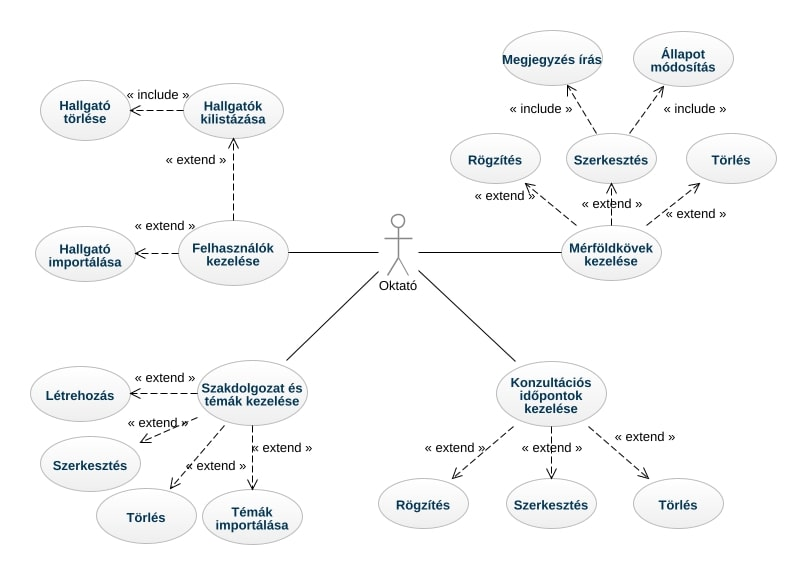
\includegraphics[width=14cm]{kepek/oktato_usecase.jpg}
		\caption{Oktató használati esetei}
		\label{fig:oktato_usecase}
	\end{figure}
	\newpage
	\subsubsection{Hallgatók}
	A hallgatói szerepkörrel rendelkező felhasználók rendelkeznek a legkevesebb jogosultsággal:
	\begin{itemize}
		\item megtekinthetik szakdolgozatuk adatlapját
		\item listázhatják az oktatójuk konzultációs időpontjait, lefoglalhatják azokat, és lemondhatják a már lefoglalt időpontokat
		\item megtekinthetik a szakdolgozatukhoz rendelt mérföldköveket
		\begin{itemize}
			\item a mérföldkövek között szűrhetnek cím, állapot szerint, rendezhetik dátum szerint
			\item megjegyzést fűzhetnek a mérföldkövekhez (fájl csatolmánnyal)
		\end{itemize}
	\end{itemize}
	\begin{figure}[!h]
		\centering
		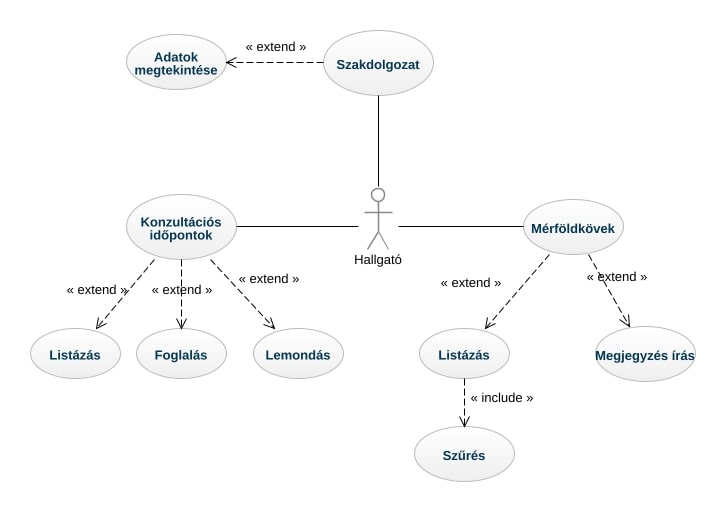
\includegraphics[width=12cm]{kepek/hallgato_usecase.jpg}
		\caption{Hallgató használati esetei}
		\label{fig:hallgato_usecase}
	\end{figure}
	\newpage
	\section{Adatbázisterv}
	Az alkalmazás által használt adatbázis megtervezése a legfontosabb lépések közé tartozik. Meg kell határozni az alkalmazásban használatos összes adatot, melyekből később a MongoDB-ben használt sémákat kell létrehozni. Ez fogja meghatározni az egyes kollekcióban tárolt adatok felépítését.
	
	A dokumentumok közötti kapcsolatok esetén (ellentétben a relációs adatbázisokkal) nem kulcsokat hozunk létre, hanem az adott sémában egy referenciát tárolunk a kapcsolni kívánt dokumentumra, mely így egy beágyazott aldokumentuma lesz az eredeti dokumentumnak. 
	
	Az adatok validálásához a sémákban minden egyes mezőre validátor metódust használhatunk, amely megadott szempontok alapján vizsgálja az adatot. Ha az adat nem felel meg a kritériumoknak, akkor hibával leáll a dokumentum létrehozása.
	
	\begin{figure}[!h]
		\centering
		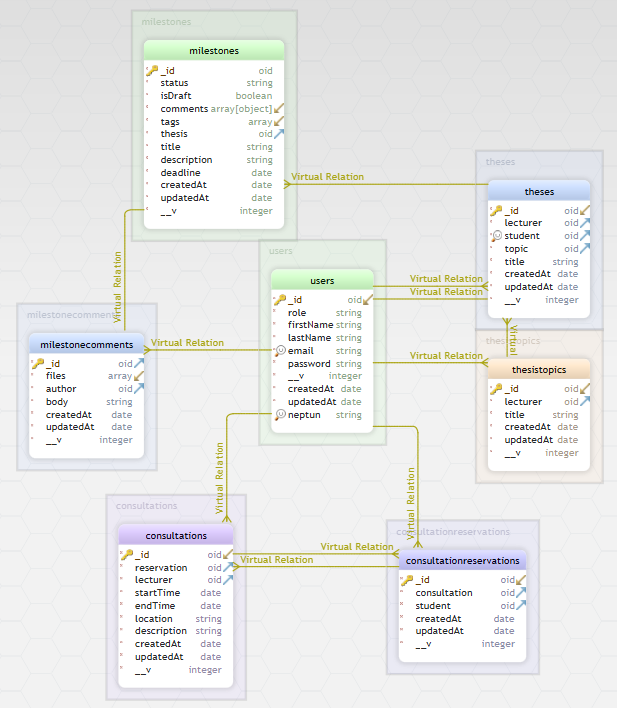
\includegraphics[width=13cm]{kepek/db_erd.png}
		\caption{A kollekciók közötti kapcsolatok}
		\label{fig:db_erd}
	\end{figure}
	\newpage
	\subsubsection{Felhasználók}
	Minden felhasználóról csupán a legfontosabb adatok kerülnek eltárolásra. Ezek a vezeték és keresztnév, NEPTUN azonosító, email cím, a belépéshez használt jelszó (hashelve) és a felhasználó jogosultsági szintje. Kikötés, hogy minden felhasználónak egyedi NEPTUN azonosítóval és email címmel kell rendelkeznie.
	
	\begin{table}[!h]
		\centering
		\begin{tabular}{|l|c|c|c|} 
			\hline
			\textbf{Mező} & \textbf{Típus} & \textbf{Hossz} & \textbf{Egyéb megkötés} \\ 
			\hline
			neptun & string & 6 karakter & UNIQUE \\ 
			\hline
			firstName & string & min. 4 karakter & - \\ 
			\hline
			lastName & string & min. 4 karakter & - \\ 
			\hline
			password & string & min. 8 karakter & - \\ 
			\hline
			email & string & - & UNIQUE \\ 
			\hline
			role & enum & - & {[}STUDENT, LECTURER, ADMIN] \\ 
			\hline
		\end{tabular}
		\caption{Felhasználó sémájának felépítése}
		\label{tbl:felhasznalo_dokumentum}
	\end{table}
	\newpage
	\subsubsection{Szakdolgozati témák}
	Minden szakdolgozati téma beágyazott aldokumentumként tárolja az oktatót, aki a témát létrehozta és a téma megnevezését.
	
	\begin{table}[!h]
		\centering
		\begin{tabular}{|l|c|c|c|} 
			\hline
			\textbf{Mező} & \textbf{Típus} & \textbf{Hossz} & \textbf{Egyéb megkötés} \\ 
			\hline
			lecturer & ObjectId & - & - \\ 
			\hline
			title & string & min. 5 karakter & - \\
			\hline
		\end{tabular}
		\caption{Szakdolgozati téma sémájának felépítése}
		\label{tbl:szakdoga_tema_dokumentum}
	\end{table}
	
	\subsubsection{Szakdolgozatok}
	Minden szakdolgozat dokumentum tartalmazza beágyazott aldokumentumként az oktatót, a hallgatót, és a szakdolgozat témáját. Minden hallgatóhoz egyetlen szakdolgozat tartozhat, ezért kikötés, hogy a hallgató referenciájának egyedinek kell lennie.
	
	\begin{table}[!h]
		\centering
		\begin{tabular}{|l|c|c|c|} 
			\hline
			\textbf{Mező} & \textbf{Típus} & \textbf{Hossz} & \textbf{Egyéb megkötés} \\ 
			\hline
			lecturer & ObjectId & - & - \\ 
			\hline
			student & ObjectId & - & UNIQUE \\ 
			\hline
			topic & ObjectId & - & - \\ 
			\hline
			title & string & min. 5 karakter & - \\
			\hline
		\end{tabular}
		\caption{Szakdolgozat sémájának felépítése}
		\label{tbl:szakdoga_dokumentum}
	\end{table}
	
	\subsubsection{Konzultációk}
	Minden egyes konzultációhoz eltárolásra kerül az oktató, akihez az időpont tartozik, a konzultáció kezdetének és végének ideje, a konzultáció helyszíne, és opcionálisan a leírás. Ezek mellett van egy mező, amely alapértelmezetten üres, viszont ha foglalás érkezik az időpontra, akkor a foglalás referenciája elmentésre kerül ebbe a mezőbe.
	
	\begin{table}[!h]
		\centering
		\begin{tabular}{|l|c|c|c|} 
			\hline
			\textbf{Mező} & \textbf{Típus} & \textbf{Hossz} & \textbf{Egyéb megkötés} \\ 
			\hline
			lecturer & ObjectId & - & - \\ 
			\hline
			startTime & Date & - & - \\ 
			\hline
			endTime & Date & - & - \\ 
			\hline
			location & string & - & - \\ 
			\hline
			description & string & - & - \\ 
			\hline
			reservation & ObjectId & - & - \\
			\hline
		\end{tabular}
		\caption{Konzultáció sémájának felépítése}
		\label{tbl:konzultacio_dokumentum}
	\end{table}
	
	\subsubsection{Konzultáció foglalások}
	A foglalások dokumentumai tartalmazzák beágyazott aldokumentumként a konzultáció és a foglaló hallgató referenciáját.
	
	\begin{table}[!h]
		\centering
		\begin{tabular}{|l|c|c|c|} 
			\hline
			\textbf{Mező} & \textbf{Típus} & \textbf{Hossz} & \textbf{Egyéb megkötés} \\ 
			\hline
			consultation & ObjectId & - & - \\ 
			\hline
			student & ObjectId & - & - \\
			\hline
		\end{tabular}
		\caption{Konzultáció foglalás sémájának felépítése}
		\label{tbl:konzultacio_foglalas_dokumentum}
	\end{table}
	
	\subsubsection{Mérföldkövek és mérföldkő megjegyzések}
	A mérföldkövek dokumentumai magában foglalják a szakdolgozat referenciáját, a mérföldkő címét és leírását, a feladat határidejét, státuszát, hogy piszkozatként van-e elmentve az adott feladat, a mérföldkőhöz tartozó megjegyzések referenciáit és az opcionálisan megadható címkék listáját.
	
	A megjegyzések dokumentumai referenciaként tárolják annak íróját, a szöveges tartalmát és az esetlegesen csatolt fájl(ok) relatív elérési útjait.
	
	\begin{table}[!h]
		\centering
		\begin{tabular}{|l|c|c|c|} 
			\hline
			\textbf{Mező} & \textbf{Típus} & \textbf{Hossz} & \textbf{Egyéb megkötés} \\ 
			\hline
			thesis & ObjectId & - & - \\ 
			\hline
			title & string & min. 3 karakter & - \\ 
			\hline
			description & string & min. 5 karakter & - \\ 
			\hline
			deadline & Date & - & - \\ 
			\hline
			status & enum & - & {[}PENDING,ACCEPTED,REJECTED] \\ 
			\hline
			isDraft & boolean & - & - \\ 
			\hline
			comments & {[}ObjectId] & - & - \\ 
			\hline
			tags & string[] & - & - \\
			\hline
		\end{tabular}
		\caption{Mérföldkő sémájának felépítése}
		\label{tbl:merfoldko_dokumentum}
	\end{table}
	
	\begin{table}[!h]
		\centering
		\begin{tabular}{|l|c|c|c|} 
			\hline
			\textbf{Mező} & \textbf{Típus} & \textbf{Hossz} & \textbf{Egyéb megkötés} \\ 
			\hline
			author & ObjectId & - & - \\ 
			\hline
			body & string & min. 3 karakter & - \\ 
			\hline
			files & string[] & - & - \\
			\hline
		\end{tabular}
		\caption{Mérföldkő megjegyzés sémájának felépítése}
		\label{tbl:merfoldko_megjegyzes_sema}
	\end{table}
	\newpage
	\section{Autentikáció és autorizáció}
	A webalkalmazás fontos és egyben legkritikusabb pontja az autentikáció. Számtalan módon lehetséges a felhasználó azonosítása, mely történhet egyedileg fejlesztett autentikációs folyamattal, de léteznek erre is előre elkészített csomagok amelyeket használhatunk. Egyik ilyen csomag a Passport.js\footnote{\url{http://www.passportjs.org/}}, melyben 500-nál is több autentikációs stratégia közül válaszhatunk, mint például: Google OAuth, Facebook, Auth0 vagy JWT\footnote{JSON Web Token}.
	
	A webalkalmazás token alapú autentikációt fog használni, nevezetesen JSON Web Token-t. A bejelentkezés során helyes email cím és jelszó párosítást megadva egy, a szerver által aláírt, és csak bizonyos időtartamig érvényes token-t kapunk válaszként, melyet minden szerver felé irányuló kérés során csatolunk a kéréshez. Minden kérés beérkezése során a szerver ellenőrzi a tokent, és ha az érvényes, akkor teljesíti a kérést.
	
	Ahogyan \az{\ref{subs:nest}}.~alfejezetben is említésre került, hogy a keretrendszerben készíthetünk Guard osztályokat, amelyeket használhatunk az autentikáció során. Az implementációhoz szükséges \emph{@nestjs/passport} csomag rendelkezik egy beépített AuthGuard nevű Guard-al, melynek paraméterben megadhatjuk az autentikáció típusát (jelen esetben jwt). Mindegyik kontroller metóduson, amelyeket csak autentikált felhasználók érhetnek el a \emph{@UseGuards()} dekorátorral alkalmaznunk kell az AuthGuard-ot, ezzel biztosítva, hogy csak és kizárólag érvényes tokennel rendelkező kérések kerüljenek kiszolgálásra.
	
	Ezen felül egyes kérések esetén szükséges vizsgálni a kérést indító felhasználó jogosultsági szintjét is. Ehhez egy saját dekorátorra (\emph{@Roles()}) és Guard-ra van szükség (\emph{RoleGuard}). A dekorátor használatával minden kontroller metódus esetén egyesével megszabhatjuk, hogy az adott erőforrást milyen jogosultsági szinttel rendelkező felhasználók érhessék el. A dekorátor egy saját metaadatban tárolja a megadott jogosultsági szinte(ke)t (\ref{kod-nest-role-metadata}.~kód).
	
	\lstinputlisting[style=user1,caption=A jogosultsági szintet tároló metaadat dekorátor,label=kod-nest-role-metadata]{kodok/role_metadata.txt}
	
	A RoleGuard ebből a metaadatból kiolvasva dönti el, hogy a kérést indító felhasználó jogosult-e a kért erőforrás elérésére (\ref{kod-nest-role-guard}.~kód).
	
	\lstinputlisting[style=user1,caption=A RoleGuard felépítése,label=kod-nest-role-guard]{kodok/role_guard.txt}
	
	A szerveroldalon kívül a kliensoldali programban is szükséges az erőforrások elérhetőségét jogosultsági szint alapján vizsgálni. Ehhez saját komponenst alkalmazhatunk, amely a store-ban eltárolt bejelentkezett felhasználó jogosultsági szintjét ellenőrzi.
	
	Ha egy bizonyos útvonalat jogosultsági szinttől függetlenül, viszont csak és kizárólag autentikált felhasználók tekinthetnek meg, úgy elegendő ellenőrzni a store-ban, hogy bejelentkezett-e a felhasználó (\ref{kod-protected-route}.~kód). Ha be van jelentkezve, akkor megjelenítjük a komponenst annak paramétereivel, ha nincs akkor átirányítjuk a felhasználót.
	
	\lstinputlisting[style=user1,caption=ProtectedRoute felépítése,label=kod-protected-route]{kodok/protected_route.txt}
	
	Amennyiben az útvonalat autentikált, és bizonyos jogosultsági szinttel rendelkező felhasználók érhetik csak el, úgy a bejelentkezés vizsgálata mellett ellenőrizni kell a belépett felhasználó jogosultsági szintjét. \Az{\ref{kod-lecturer-route}}.~kódban látható komponens csak azon felhasználóknak engedélyezi az útvonal elérést, amelyek oktatói jogosultsággal rendelkeznek.
	
	\lstinputlisting[style=user1,caption=LecturerRoute felépítése,label=kod-lecturer-route]{kodok/lecturer_route.txt}
	
	\section{Kliensoldali alkalmazás felépítése}
	Révén, hogy az alkalmazásnak többféle jogosultsági szinttel rendelkező felhasználókat kell kiszolgálnia, így a kliensoldali React alkalmazást két kisebb alkalmazásra bontom föl. Egyik az ügyintézői, a másik pedig az oktatói és hallgatói modul. Ennek előnye, hogy a két rendszer elkülönül egymástól, mindkettő saját útválasztással és Redux állapotkezeléssel rendelkezik. Ezáltal egyszerűbb a külön-külön modulokban való fejlesztés, nem lesz túlságosan összetett és bonyolult a mögöttes Redux állapot felépítése.
	
	A React alkalmazás fő App komponensének szerepe mindössze annyi, hogy elkülönítse az ügyintézői, oktatói, hallgatói, és a hibaútvonalakat (például \emph{,,404 - Az oldal nem található''}). Az ezeken belüli navigálás a továbbiakban már az adott modul feladata. 
	
	A mindkét modul által használt komponensek, Redux által használt action és reducer fájlok a projekt gyökérmappájában található közös mappában helyezkednek el. Innen mindkét modulból elérhetőek, újrafelhasználhatóak, ezáltal elkerülve a fölösleges kódismétléseket.
	
	A Redux store minden oldalfrissítéssel kiürül, ez az autentikáció szempontjából hátrányos, ugyanis minden oldalfrissítéssel újra és újra le kellene kérni a szervertől a felhasználó tokenje alapján a felhasználó adatait. Hogy ezt a problémát kiküszöböljem a \emph{redux-persist}\footnote{\url{https://github.com/rt2zz/redux-persist}} csomagot fogom használni. Ez egy olyan köztes funkció szerepét tölti be, amely megadott reducer-ek esetében a store-ban tárolt adatokról egy másolatot tárol a böngésző lokális tárolójában (localStorage vagy sessionStorage). Oldalfrissítés esetén pedig innen visszatöltődnek az adatok a store-ba.
	
	\chapter{Fejlesztői dokumentáció}
	\Az{\ref{chp:specifikacio}}.~fejezetben leírt tervek alapján a webalkalmazás a belépett felhasználó jogosultsági szintjének megfelelő felhasználói interfészt biztosít. Az alkalmazás háromféle jogosultsági szint kezelésére képes: ügyintéző, oktató és hallgató. A felületek hozzáférése előtt a felhasználónak be kell jelentkeznie a fiókjához tartozó email címmel és jelszavával.
	
	\begin{figure}[!h]
		\centering
		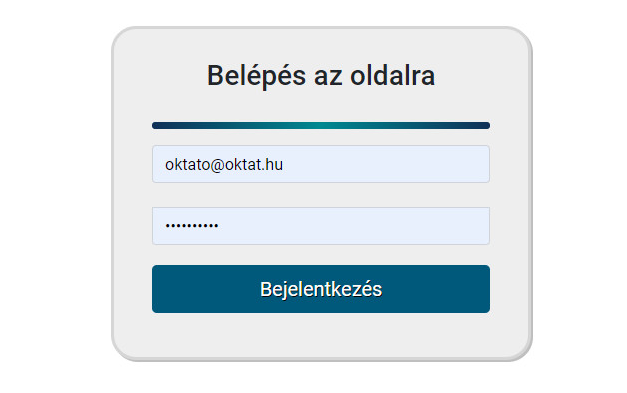
\includegraphics[width=8cm]{kepek/screenshots/belepes.png}
		\caption{Felhasználói belépő felület}
		\label{fig:belepes}
	\end{figure}
	
	\begin{figure}[!h]
		\centering
		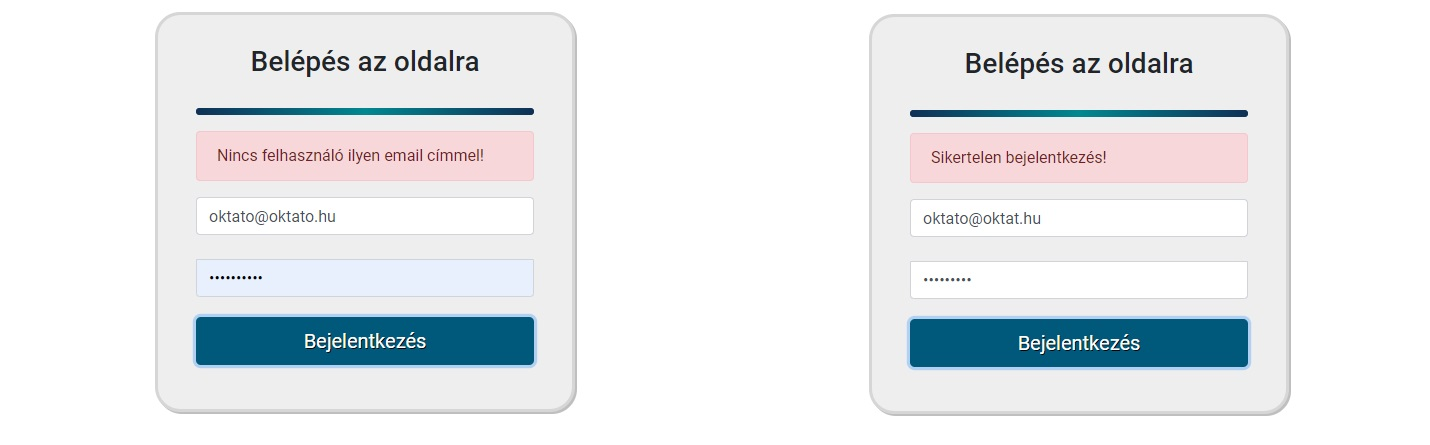
\includegraphics[width=15cm]{kepek/screenshots/sikertelen_belepes.jpg}
		\caption{Sikertelen belépés esetén hibaüzenet kerül kiírásra}
		\label{fig:sikertelen_belepes}
	\end{figure}
	
	Sikeres bejelentkezést követően a menüsor jobb szélén megjelenő \emph{,,Teljes név (Jogosultság)''} lenyíló menüre kattintva megtekintheti a felhasználó a profil beállításait (profil adatlap és jelszóváltoztatás), illetve kijelentkezhet a felületről, amennyiben nem szeretné azt tovább használni.
	
	\begin{figure}[!h]
		\centering
		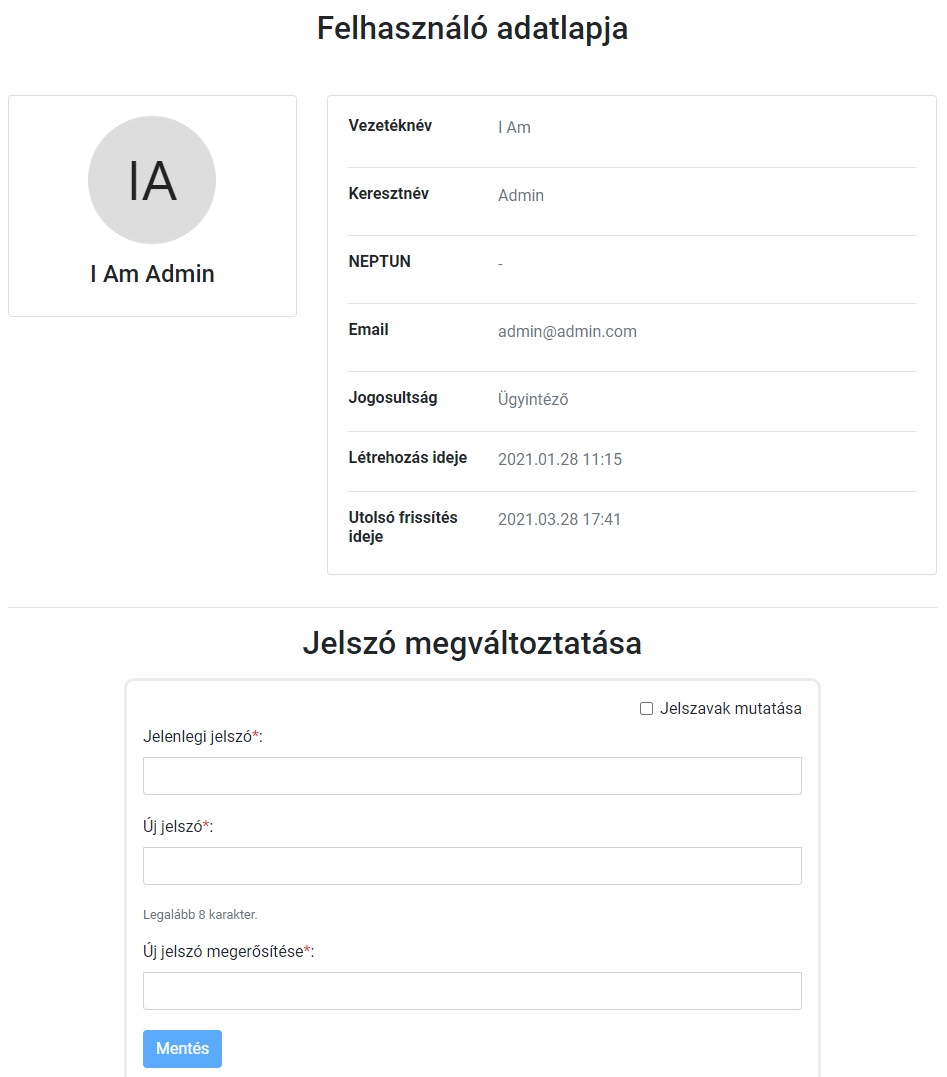
\includegraphics[width=15cm]{kepek/screenshots/ugyintezo_beallitasok.png}
		\caption{Felhasználó adatlap és jelszómódosítás}
		\label{fig:ugyint_felhasznalo_profil}
	\end{figure}
	
	\section{Ügyintézői felület}
	A rendszer használatára jogosult felhasználókat az ügyintézők saját felületükön tudják kezelni. A sikeres bejelentkezés után alapértelmezetten a hallgatók kerülnek kilistázásra táblázatos formában, a menüsorban elérhető \emph{,,Oktatók''} és \emph{,,Ügyintézők''} menüpontokban lehetőség van az ezekkel a jogosultságokkal rendelkező felhasználók menedzselésére is.
	
	\Az{\ref{fig:ugyint_hallgatok}}.~ábrán látható táblázat a szűrésen kívül két további funkcióval rendelkezik: az adott felhasználó adatlapjának megjelenítésére szolgáló kék ikonnal, illetve a felhasználó törlésére szolgáló piros ikonnal. A törlés ikonra kattintva egy felugró ablakban kell megerősítenie az ügyintézőnek a felhasználó törlésének szándékát.
	
	\begin{figure}[!h]
		\centering
		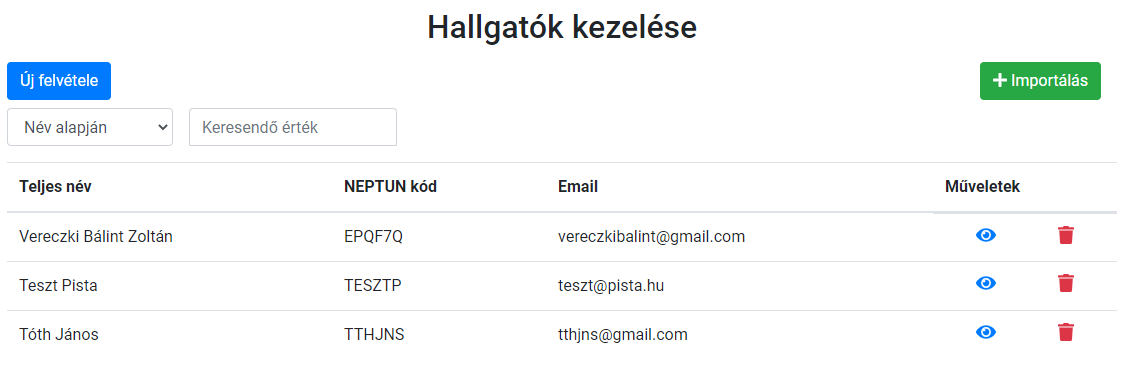
\includegraphics[width=15cm]{kepek/screenshots/ugyintezo_hallgatok.png}
		\caption{Hallgatók listája}
		\label{fig:ugyint_hallgatok}
	\end{figure}
	
	A táblázatban szereplő felhasználók szűrése a lenyíló menüben található szempontok (név, email, NEPTUN azonosító) alapján lehetséges, a \emph{,,Keresendő érték''} mezőbe írt érték alapján. A webalkalmazás többféle módot is biztosít az ügyintézők számára, hogy új felhasználókat vigyenek fel a rendszerbe: az \emph{,,Új felvétele''} feliratú gombra kattintva \az{\ref{fig:ugyint_felhasznalo_form}}.~ábrán látható űrlap kitöltésével egy felhasználót, az \emph{,,Importálás''} feliratú gombra kattintva CSV formátumú adatforrásból képes egyszerre több felhasználót felvinni a rendszerbe. 
	
	\begin{figure}[!h]
		\centering
		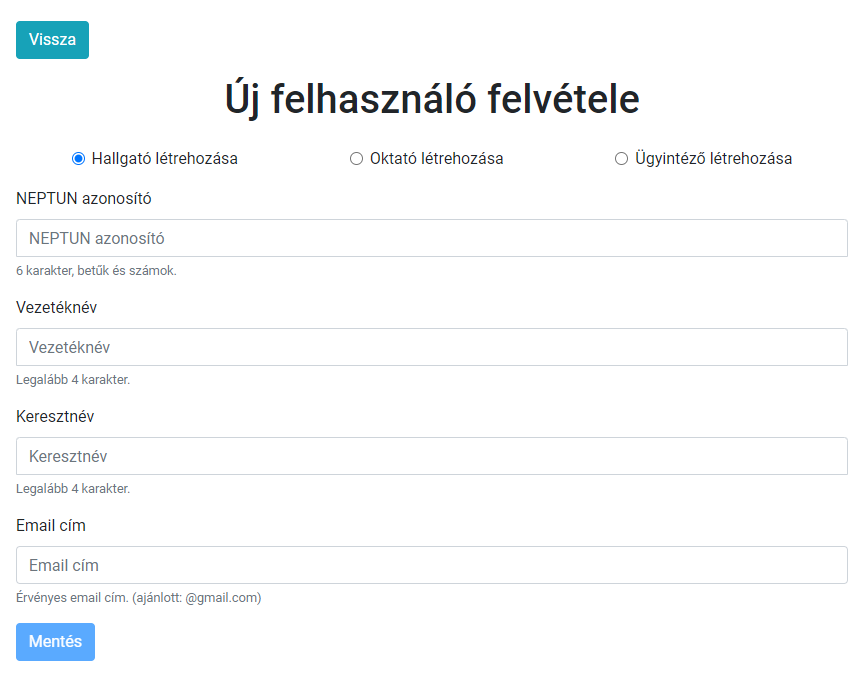
\includegraphics[width=10cm]{kepek/screenshots/ugyintezo_uj_felhasznalo.png}
		\caption{Új felhasználó felvitele űrlap segítségével}
		\label{fig:ugyint_felhasznalo_form}
	\end{figure}
	
	Felhasználók importálására kizárólag pontosvesszővel tagolt, maximum 1 megabájt méretű CSV formátumból van lehetőség, hiba esetén \az{\ref{fig:ugyint_felhasznalo_import_hiba}}.~ábrán látható hibaüzenet jelenik meg.
	
	\begin{figure}[!h]
		\centering
		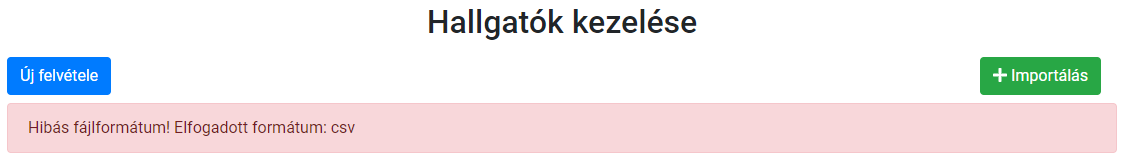
\includegraphics[width=15cm]{kepek/screenshots/ugyintezo_felhasznalo_import_hiba.png}
		\caption{Sikertelen felhasználó importálás}
		\label{fig:ugyint_felhasznalo_import_hiba}
	\end{figure}
	
	A táblázatban a kék ikonra kattintva megnyílik a hallgató adatlapja és megjelenik minden fontos információ az adott felhasználóról, úgy mint a neve, NEPTUN azonosítója, email címe, jogosultsági szintje, a profil létrehozásának és legutolsó frissítésének pontos ideje. Az adatlap fölött jobb oldalon található \emph{,,Szerkesztés''} feliratú gomb megnyomásával átvált az oldal szerkesztői módba, a szerkeszthető mezők beviteli mezővé alakulnak át. A szerkesztést az adatlap fölött középen található \emph{,,Mentés''} feliratú gombbal lehet véglegesíteni, ha nem kívánjuk menteni az adatokat, akkor a szerkesztést a \emph{,,Mégsem''} feliratú gombra kattintva fejezhetjük be.
	
	\begin{figure}[!ht]
		\centering
		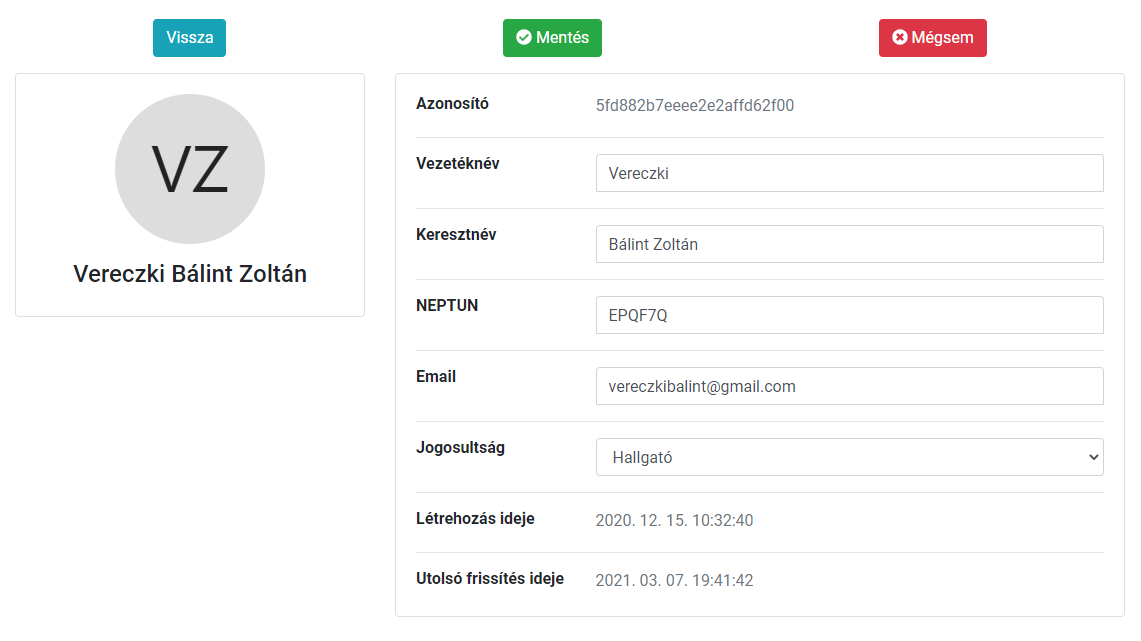
\includegraphics[width=12cm]{kepek/screenshots/ugyintezo_felhasznalo_szerkesztes.png}
		\caption{Felhasználó szerkesztése}
		\label{fig:ugyint_felhasznalo_szerkesztes}
	\end{figure}
	
	A szerkesztés során felmerülő hibákról (mint a már regisztrált NEPTUN kód és email cím) a Mentés gombra kattintás után kap visszajelzést a felhasználó (\ref{fig:ugyint_felhasznalo_szerkesztes_hiba}.~ábra), ilyenkor a beviteli mező piros körvonallal jelenik meg, benne egy felkiáltójel ikonnal, a mező alatt pedig piros felirattal jelenik meg a mezőre vonatkozó hibaüzenet.
	
	\begin{figure}[!ht]
		\centering
		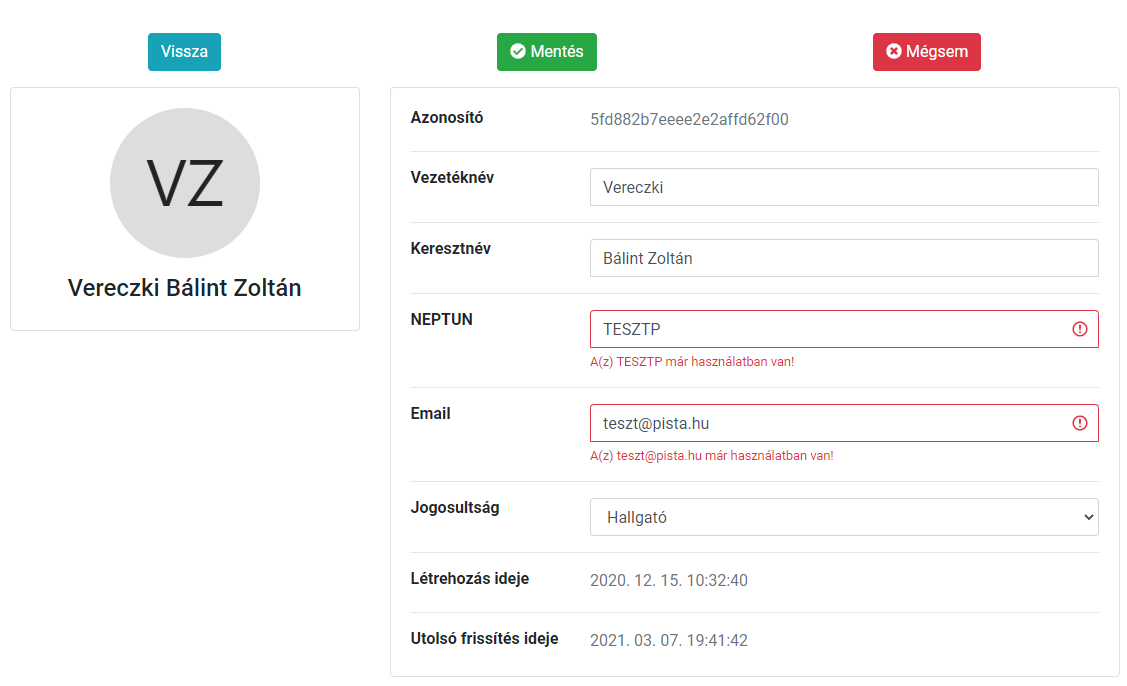
\includegraphics[width=12cm]{kepek/screenshots/ugyintezo_felhasznalo_szerkesztes_hiba.png}
		\caption{Szerkesztés során felmerülő hibák}
		\label{fig:ugyint_felhasznalo_szerkesztes_hiba}
	\end{figure}
	
	\section{Oktatói felület}
	\subsection{Szakdolgozatok és témák}
	Sikeres bejelentkezést követően alapértelmezetten a \emph{,,Szakdolgozatok kezelése''} oldal fogadja az oktatót. Amennyiben még az adott oktatóhoz nem került rögzítésre szakdolgozat akkor a \emph{,,Nincsen szakdolgozat az adatbázisban''} hibaüzenet jelenik meg (\ref{fig:oktato_szakdolgozat_nincs}.~ábra), ellenkező esetben pedig táblázatos formában az összes szakdolgozat (\ref{fig:oktato_szakdolgozat_tablazat}.~ábra). A táblázat fölött található szűrők segítségével lehet keresni a szakdolgozatok között, hallgató neve, téma és a szakdolgozat címe alapján.
	
	\begin{figure}[!h]
		\centering
		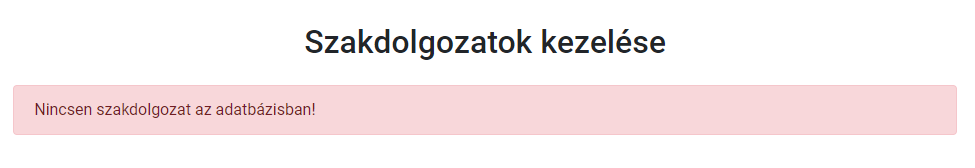
\includegraphics[width=12cm]{kepek/screenshots/oktato_szakdolgozat_nincs.png}
		\caption{Hibaüzenet, ha nincsen szakdolgozat rögzítve}
		\label{fig:oktato_szakdolgozat_nincs}
	\end{figure}
	
	Szakdolgozat rögzítése előtt rögzíteni kell a rendszerben a szakdolgozati témákat, melyet a \emph{,,Szakdolgozati témák''} menüpontja alatt lehet megtenni többféle módon (\ref{fig:oktato_tema_kezeles}.~ábra). Ha csak egy-egy téma felvitelére van szükség, akkor a bal oldali beviteli mezőbe begépelve felvihető, több téma esetén pedig a jobb oldali \emph{,,Importálás''} gombra kattintva pontosvesszővel tagolt CSV fájlból lehet importálni. A téma szerkesztésére és törlésére az adott téma sorának végén található ikonokra kattintva van lehetőség.
	
	\begin{figure}[!h]
		\centering
		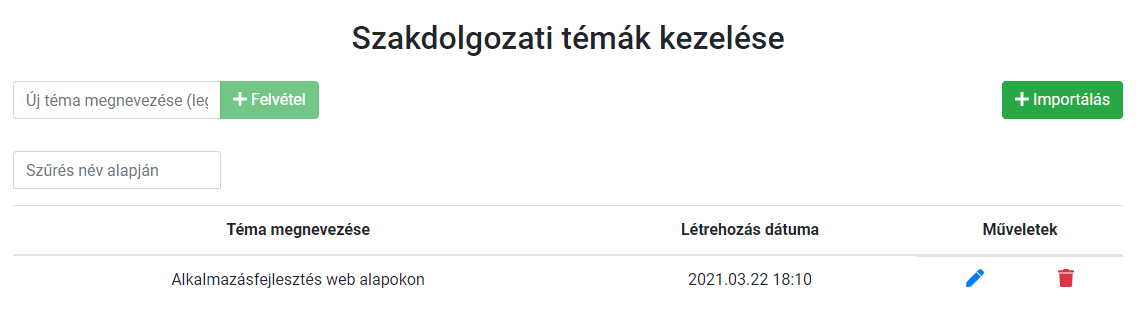
\includegraphics[width=12cm]{kepek/screenshots/oktato_tema_kezeles.png}
		\caption{Szakdolgozati témák kezelése}
		\label{fig:oktato_tema_kezeles}
	\end{figure}
	\newpage
	Szakdolgozat rögzítésére a \emph{,,Szakdolgozat''} lenyíló menüben található \emph{,,Új létrehozása''} menüpont alatt van lehetőség (\ref{fig:oktato_szakdolgozat_letrehozas}.~ábra). Ha a rendszerben még nem szerepelnek hallgatók vagy az oktatóhoz tartozó szakdolgozati témák, úgy a beviteli mezők letiltásra kerülnek. Ellenkező esetben a mezőbe kattintva megjelennek az elérhető értékek, melyek között a mezőbe való gépeléssel lehet keresni. Ha a kiválasztott hallgatóhoz már hozzá van rendelve egy szakdolgozat, akkor a beviteli mező alatt \emph{,,Ehhez a hallgatóhoz már tartozik szakdolgozat!''} hibaüzenet kerül megjelenítésre.
	
	\begin{figure}[!h]
		\centering
		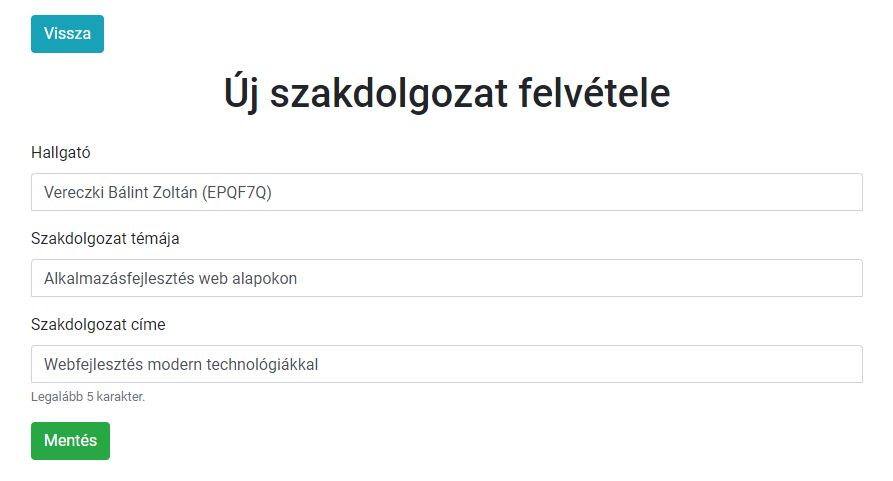
\includegraphics[width=12cm]{kepek/screenshots/oktato_szakdolgozat_letrehozas.png}
		\caption{Szakdolgozat létrehozása}
		\label{fig:oktato_szakdolgozat_letrehozas}
	\end{figure}
	
	\begin{figure}[!h]
		\centering
		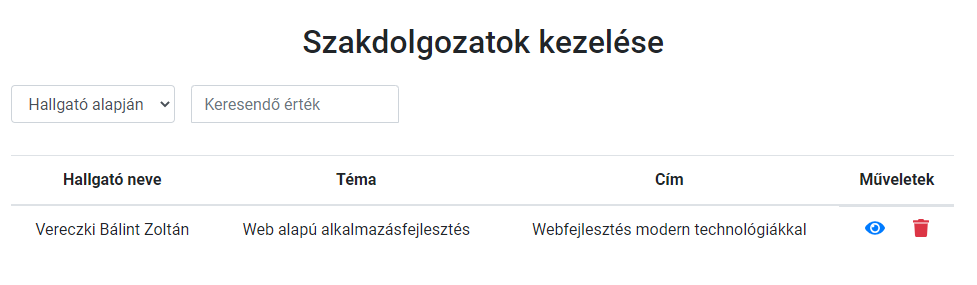
\includegraphics[width=12cm]{kepek/screenshots/oktato_szakdolgozat_tablazat.png}
		\caption{Szakdolgozatok táblázatos formában}
		\label{fig:oktato_szakdolgozat_tablazat}
	\end{figure}
	
	A táblázat két művelet elvégzésére nyújt opciót: a szakdolgozat adatlapjának és szerkesztő felületének megnyitására (\ref{fig:oktato_szakdolgozat_adatlap}.~ábra), és a szakdolgozat törlésére, amely egy felugró ablakban történő megerősítés után történik meg.
	
	\begin{figure}[!h]
		\centering
		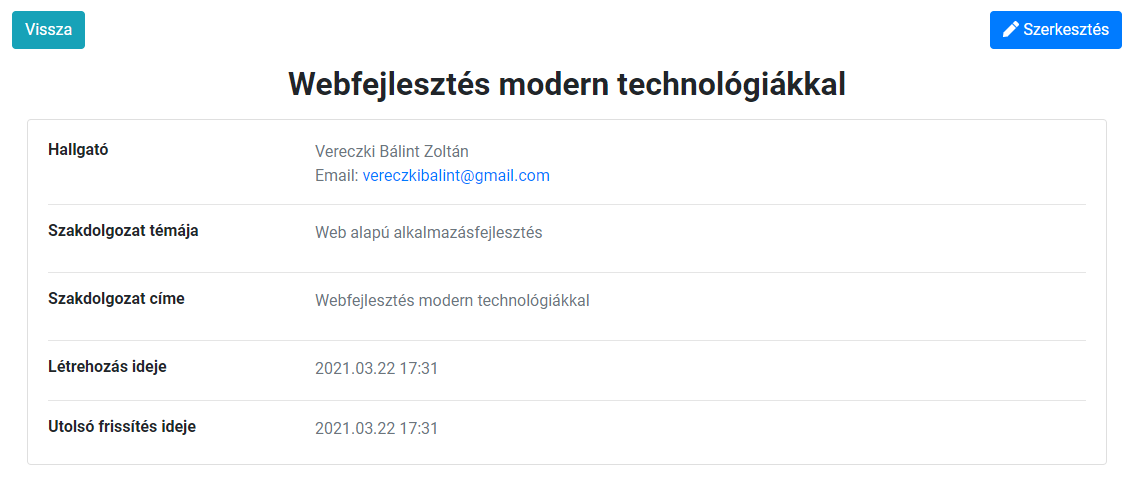
\includegraphics[width=11cm]{kepek/screenshots/oktato_szakdolgozat_adatlap.png}
		\caption{Szakdolgozat adatlapja}
		\label{fig:oktato_szakdolgozat_adatlap}
	\end{figure}
	
	Az adatlapon a jobb felső sarokban található \emph{,,Szerkesztés''} feliratú gombra kattintva átvált az oldal szerkesztői módba (\ref{fig:oktato_szakdolgozat_szerkesztes}.~ábra), ahol lehetőség van a szakdolgozat hallgatóját, témáját és címét megváltoztatni.
	
	\begin{figure}[!h]
		\centering
		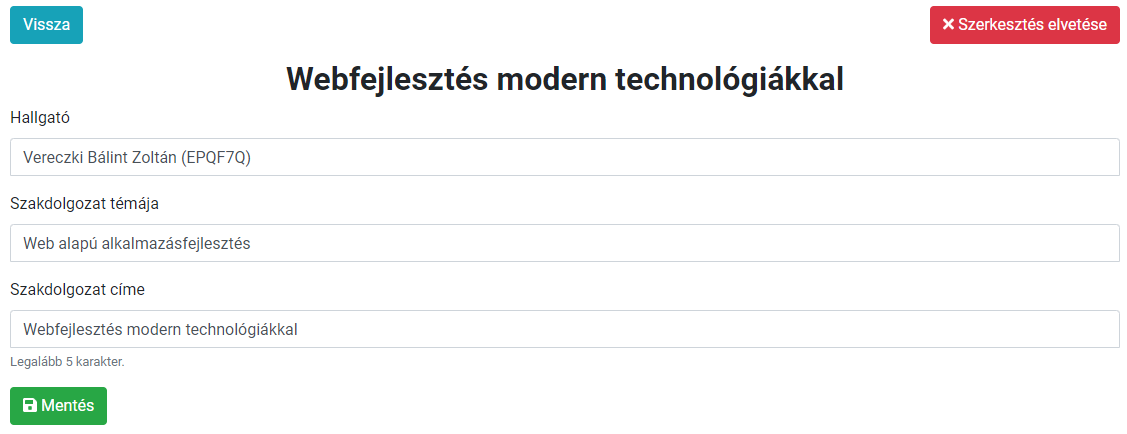
\includegraphics[width=11cm]{kepek/screenshots/oktato_szakdolgozat_adatlap_szerkesztes.png}
		\caption{Szakdolgozat szerkesztése}
		\label{fig:oktato_szakdolgozat_szerkesztes}
	\end{figure}
	
	\subsection{Hallgatók}
	A \emph{,,Hallgatók''} menüpont alatt elérhető felületen tudják az oktatók menedzselni a rendszerbe rögzített hallgatókat. Ha valamilyen adatra van szükség, akkor a felhasználó adatlapját megtekinthetik, illetve törölhetik is az adott hallgató profilját a rendszerből. Lehetőség van név, NEPTUN azonosító és email cím szerint szűrni az adatokat, illetve pontosvesszővel tagolt CSV fájlból új hallgatókat felvinni a rendszerbe.
	
	\begin{figure}[!h]
		\centering
		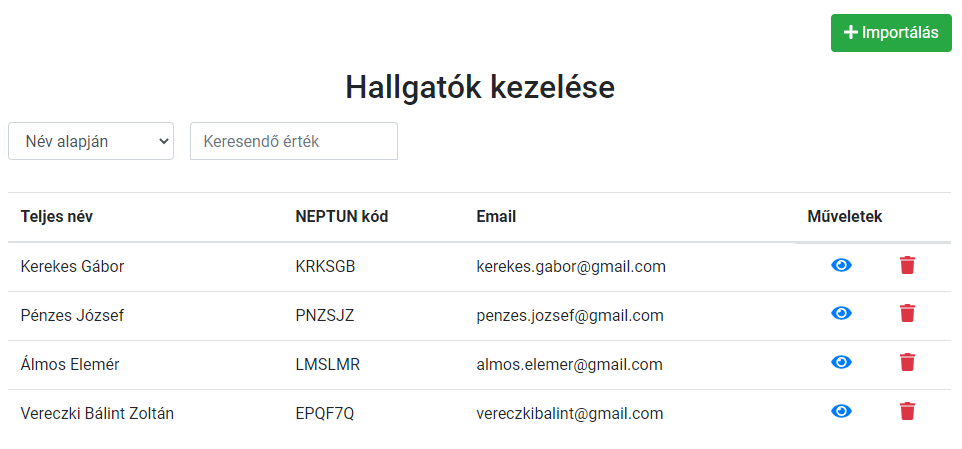
\includegraphics[width=12cm]{kepek/screenshots/oktato_hallgato_kezeles.png}
		\caption{Hallgatók kezelése}
		\label{fig:oktato_hallgato_kezelese}
	\end{figure}
	\newpage
	\subsection{Konzultációk}
	A \emph{,,Konzultációk''} menüpont alatt kezelhetőek a kiírt konzultációk, és megtekinthető, hogy egyes időpontokat mely hallgatók foglalták le.
	
	Amennyiben az oktató még nem rögzített konzultációs időpontot a rendszerbe, úgy a \emph{,,Nem található konzultáció!''} hibaüzenet jelenik meg az oldalon.
	
	A \emph{,,Konzultációk''} lenyíló menüben az \emph{,,Új létrehozása''} menüpont alatt hozható létre egy új konzultációs időpont  (\ref{fig:oktato_konzultacio_letrehozas}.~ábra). A létrehozás során kötelező a konzultációs időpont kezdetét és végét, illetve a helyszínét megadni. A \emph{,,Leírás''} mező opcionálisan kitölthető, melyben kiegészítő információk adhatóak meg az eseményhez (például online konzultáció esetén Zoom meghívó / konferencia csatlakozáshoz szükséges link).
	
	\begin{figure}[!h]
		\centering
		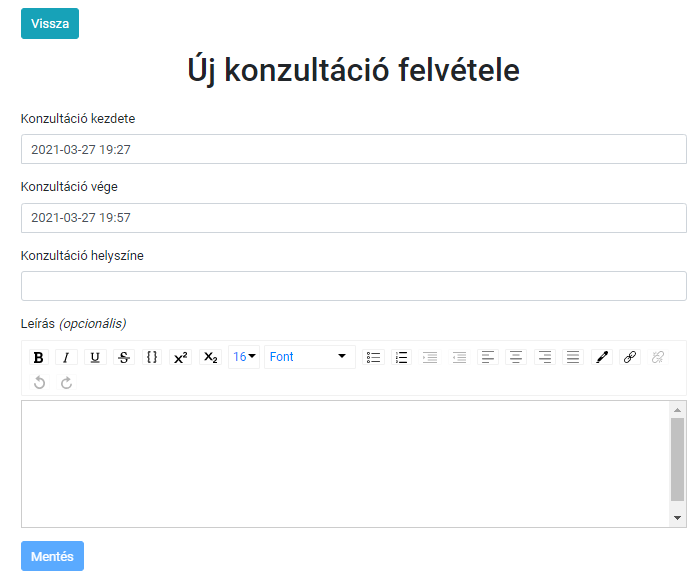
\includegraphics[width=10cm]{kepek/screenshots/oktato_konzultacio_letrehozas.png}
		\caption{Új konzultációs időpont létrehozása}
		\label{fig:oktato_konzultacio_letrehozas}
	\end{figure}
	
	A konzultációk listázása oldalon megtekinthető az összes rögzített időpont azok leírásával, és elérhetőségének állapotával (elérhető állapot esetén egy zöld pipa ikonnal, foglalt állapotban pedig a foglaló hallgató nevével és NEPTUN azonosítójával, \ref{fig:oktato_konzultacio_lista}.~ábra). Ezen kívül a sorok végén található ikonokkal szerkeszthetőek és törölhetőek az időpontok.
	
	\begin{figure}[!h]
		\centering
		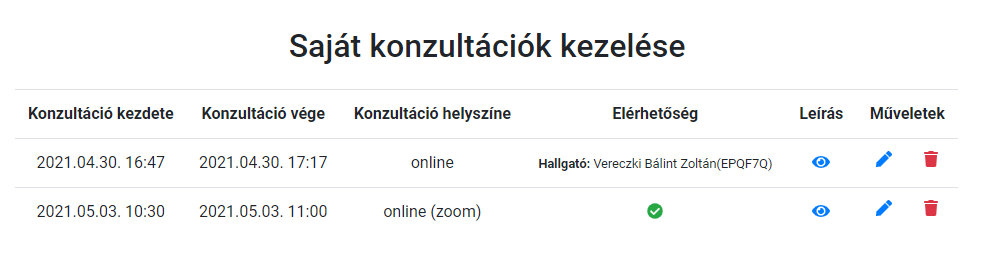
\includegraphics[width=11cm]{kepek/screenshots/oktato_konzultacio_tablazat_tobb.png}
		\caption{Konzultációk listája}
		\label{fig:oktato_konzultacio_lista}
	\end{figure}
	
	\subsection{Mérföldkövek}
	A \emph{,,Mérföldkövek''} menüpont alatt kezelhető minden szakdolgozathoz rendelt mérföldkő. A listázó oldalon a \emph{,,Szakdolgozat''} lenyíló menüben választható ki, hogy melyik szakdolgozathoz tartozó mérföldkövek kerüljenek kilistázásra. Amennyiben az adott szakdolgozathoz nem tartozik mérföldkő, úgy a \emph{,,A megadott kritériumokkal nem található mérföldkő!''} hibaüzenet kerül kiírásra (\ref{fig:oktato_merfoldko_lista_nincs}.~ábra).
	
	\begin{figure}[!h]
		\centering
		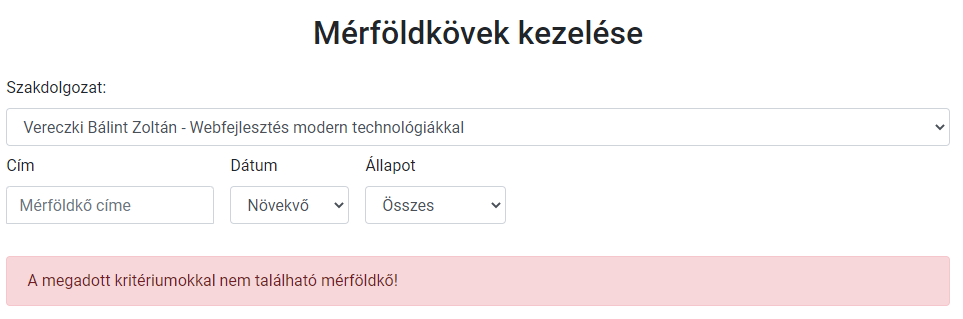
\includegraphics[width=12cm]{kepek/screenshots/oktato_merfoldko_lista_nincs.png}
		\caption{Hibaüzenet, amennyiben nincs rögzített mérföldkő}
		\label{fig:oktato_merfoldko_lista_nincs}
	\end{figure}
	
	A kilistázott mérföldkövek (\ref{fig:oktato_merfoldko_lista}.~ábra) rendezése és az azok közötti szűrés a szakdolgozat választó menü alatti opciókkal tehető meg. Az adatok szűrhetőek cím alapján, és állapotuk alapján (Folyamatban, Elfogadott, Elutasított), illetve határidejük alapján rendezhetőek növekvő és csökkenő sorrendben (alapértelmezetten csökkenő sorrendben jelennek meg). 
	
	\begin{figure}[!h]
		\centering
		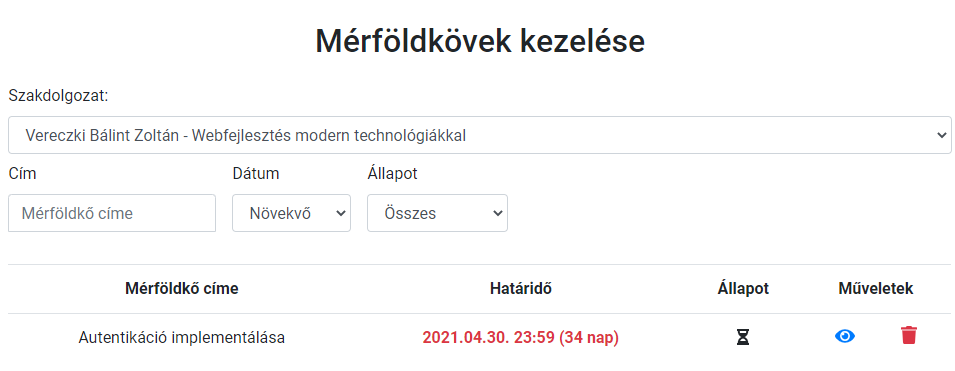
\includegraphics[width=12cm]{kepek/screenshots/oktato_merfoldko_lista.png}
		\caption{Mérföldkövek kilistázva}
		\label{fig:oktato_merfoldko_lista}
	\end{figure}
	
	Azon mérföldkövek határideje, melyek még nem jártak le, vastag, piros betűszínnel jelennek meg. A feladat állapota az annak megfelelő ikonnal jelenik meg (Folyamatban esetén homokóra, Elfogadott esetén zöld pipa, Elutasított esetén piros x ikonnal).
	
	A sor végén található kék szem ikonnal nyitható meg a mérföldkő adatlapja, ahol elolvasható a feladat részletes leírása, módosítható a feladat állapota, illetve hozzászólások formájában kommunikálhat az oktató a hallgatóval, ahol csatolmány formájában segédanyagokat, dokumentumokat és egyéb fájlokat oszthatnak meg egymással.
	
	A mérföldkő adatlapjának (\ref{fig:oktato_merfoldko_adatlap}.~ábra) jobb oldalán elhelyezkedő \emph{,,Szerkesztés''} feliratú gombra kattintva váltható az oldal szerkesztő módba. Ekkor az oldal aljáról eltűnik a \emph{,,Megjegyzések''} szekció, a részletes leírás helyén pedig megjelenik a szerkesztési űrlap, ahol megváltoztatható a feladat címe, határideje, leírása és a címkéi.
	
	A szerkesztés gomb alatt változtatható meg a feladat állapota, a háttérszínnel kijelölt gomb mutatja a feladat jelenlegi állapotát. Állapotváltoztatás esetén egy új komment jön létre a \emph{,,Megjegyzések''} szekcióban, amely rögzíti az új állapotot, és leolvasható a komment dátumáról a változtatás időpontja.
	
	\begin{figure}[!h]
		\centering
		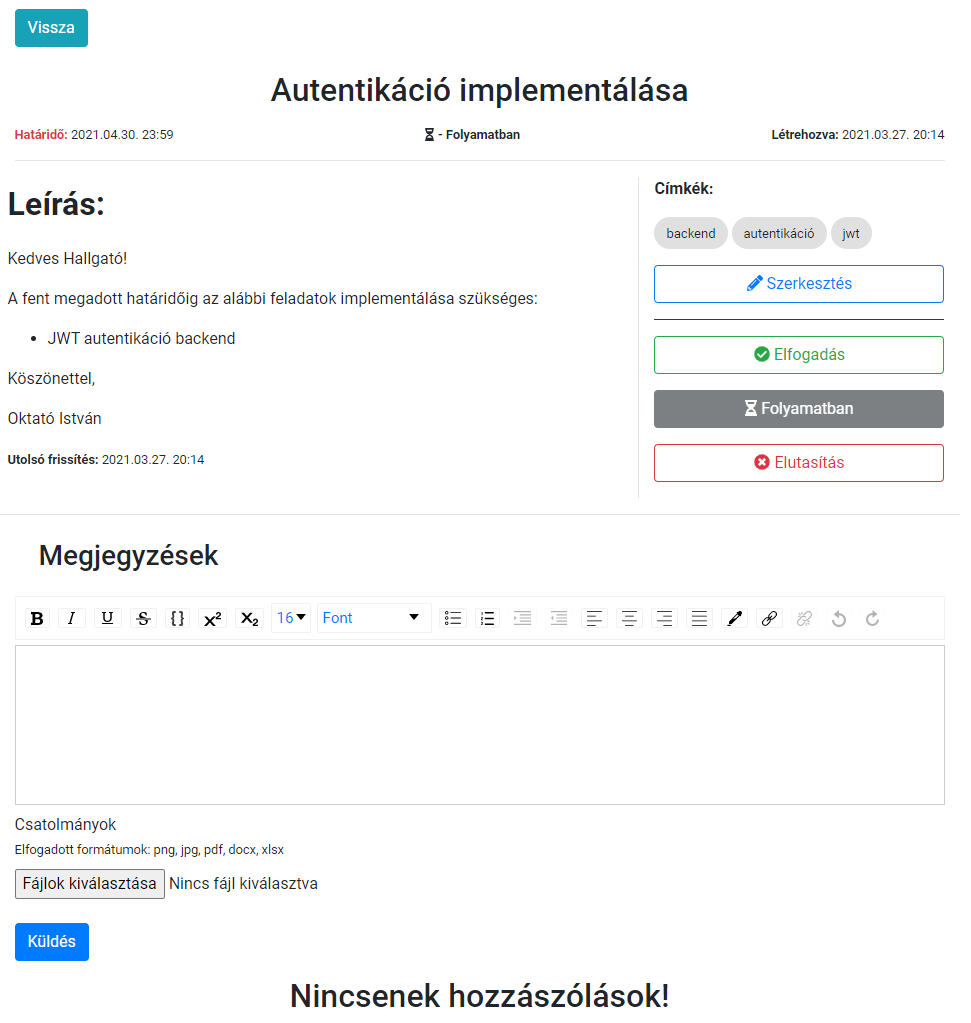
\includegraphics[width=11.5cm]{kepek/screenshots/oktato_merfoldko_adatlap.png}
		\caption{Egy mérföldkő adatlapja}
		\label{fig:oktato_merfoldko_adatlap}
	\end{figure}
	
	Mérföldkövet létrehozni a \emph{,,Mérföldkövek''} lenyíló menüben található \emph{,,Új létrehozása''} menüpont alatt elérhető űrlap kitöltésével lehet (\ref{fig:oktato_merfoldko_letrehozas}.~ábra). A ,,Szakdolgozat'' lenyíló menüből kiválasztható, hogy mely hallgató mely szakdolgozatához szeretnénk a mérföldkövet rögzíteni. Ha még nincsen az oktatóhoz rendelve szakdolgozat, akkor a menü letiltásra kerül (nem lesz kattintható), és a \emph{,,Nincs elérhető szakdolgozat!''} felirat jelenik meg a menüben.
	
	A mérföldkő címén és határidején kívül opcionálisan megadhatóak kulcsszavak, másnéven címkék is, melyekhez segítséget a \emph{,,Címkék''} felirat melletti kérdőjel ikonra kattintva lehet elolvasni. Ezek a kulcsszavak segítenek a hallgatónak az adott témában való keresésben. Címke rögzítése az Enter billentyű lenyomása után történik meg, törlésre pedig használható a címke mellett megjelenő ,,X'' ikon, vagy kétszer egymás után leütött Backspace billentyű is.
	
	A rendszer lehetőséget nyújt a mérföldkövek piszkozatként való mentésére is, amely a \emph{,,Mentés piszkozatként''} gombra kattintva tehető meg. Ekkor a piszkozat megtekinthető, a továbbiakban szerkeszthető és törölhető is az oktató által, viszont a hallgató számára nem jelenik meg. Az oktatói felületen a piszkozatként mentett mérföldkövek neve pirossal jelenik meg, zárójelben a ,,piszkozat'' szóval megjelölve. Ahhoz, hogy egy piszkozatnak jelölt mérföldkő megjelenjen a hallgató számára is a mérföldkő szerkesztői módjában a \emph{,,Közzététel''} gombra kattintva kell elmenteni a feladatot.
	
	\begin{figure}[!h]
		\centering
		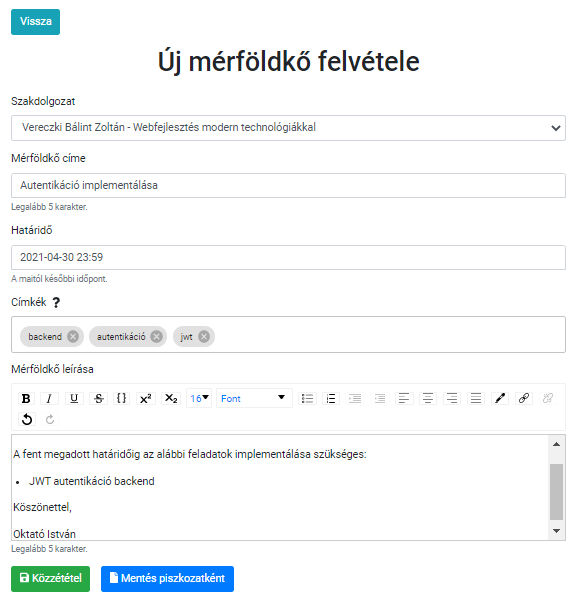
\includegraphics[width=11cm]{kepek/screenshots/oktato_merfoldko_letrehozas.png}
		\caption{Mérföldkő létrehozása}
		\label{fig:oktato_merfoldko_letrehozas}
	\end{figure}

	\newpage
	
	\section{Hallgatói felület}
	\subsection{Szakdolgozat}
	A hallgató bejelentkezése után alapértelmezetten a \emph{,,Szakdolgozat''} oldal jelenik meg. Amennyiben az adott hallgatóhoz még nincsen szakdolgozat rendelve úgy a \emph{,,Nincsen szakdolgozat az Ön felhasználójához rendelve!''} hibaüzenet jelenik meg (\ref{fig:hallgato_szakdolgozat_nincs}.~ábra).
	
	\begin{figure}[!h]
		\centering
		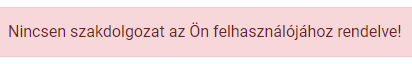
\includegraphics[width=8cm]{kepek/screenshots/hallgato_szakdolgozat_nincs.png}
		\caption{A hallgatóhoz nincsen szakdolgozat rendelve}
		\label{fig:hallgato_szakdolgozat_nincs}
	\end{figure}
	
	Amennyiben a hallgatóhoz már van szakdolgozat rendelve, úgy annak adatlapja jelenik meg (\ref{fig:hallgato_szakdolgozat_adatlap}.~ábra). Az adatlapon az oktató nevén és email elérhetőségén kívül leolvasható a szakdolgozat témája, címe, a mérföldkövek száma státuszonkénti lebontásban, és a szakdolgozat rögzítésének, illetve legutóbbi frissítésének pontos ideje.
	
	\begin{figure}[!h]
		\centering
		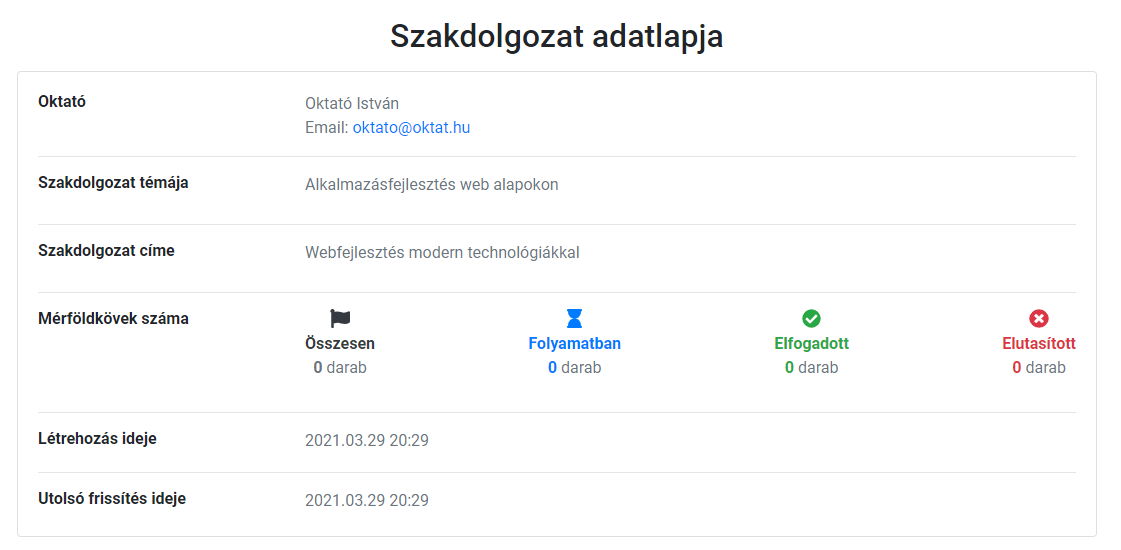
\includegraphics[width=12cm]{kepek/screenshots/hallgato_szakdolgozat_adatlap.png}
		\caption{Szakdolgozat adatlapja}
		\label{fig:hallgato_szakdolgozat_adatlap}
	\end{figure}
	
	\subsection{Konzultációk}
	A \emph{,,Konzultációk''} menüpont alatt lekérdezhető a hallgatók által a szakdolgozati oktatójuk összes konzultációs időpontja, illetve megtekinthető azok elérhetősége.
	
	Ha a hallgatóhoz nincsen még szakdolgozat rögzítve, akkor a \emph{,,Konzultációk lekérése nem lehetséges!''} hibaüzenet jelenik meg az oldalon (\ref{fig:hallgato_konzultacio_nincs_szakdolgozat}.~ábra). Ha van a hallgatóhoz szakdolgozat rendelve, de az oktatónak nincsen konzultációs időpontja a rendszerbe rögzítve, akkor a \emph{,,A megadott feltételekkel nincs elérhető konzultáció!''} hibaüzenet jelenik meg.
	
	A konzultációs időpontok megjelenítési módjára két opció közül lehet választani: az összes időpont kilistázása, illetve a hallgató által lefoglalt időpontok megjelenítése (\ref{fig:hallgato_konzultacio_idopontok}.~ábra). Ha a hallgató még nem foglalt le egyetlen időpontot sem, akkor a \emph{,,A megadott feltételekkel nincs elérhető konzultáció!''} hibaüzenet jelenik meg az oldalon.
	
		\begin{figure}[!h]
		\centering
		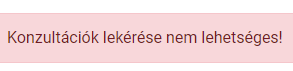
\includegraphics[width=6cm]{kepek/screenshots/hallgato_konzultacio_nincs_szakdolgozat.png}
		\caption{Hibaüzenet, ha a hallgatóhoz nem tartozik szakdolgozat}
		\label{fig:hallgato_konzultacio_nincs_szakdolgozat}
	\end{figure}
	
	\begin{figure}[!h]
		\centering
		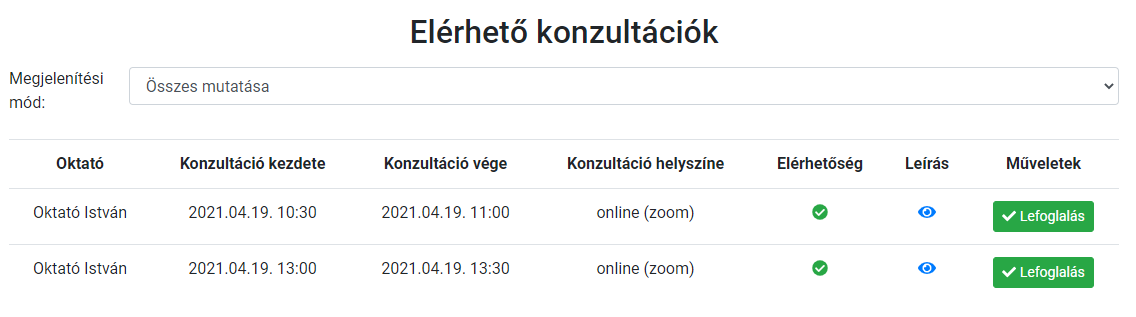
\includegraphics[width=12cm]{kepek/screenshots/hallgato_konzultacio_idopontok.png}
		\caption{Konzultációs időpontok listája}
		\label{fig:hallgato_konzultacio_idopontok}
	\end{figure}
	
	Minden konzultációhoz megjelenik a kezdet és befejezés időpontja, a konzultáció helyszíne, és az időpont elérhetősége. Ha az időpont még nincsen lefoglalva, akkor egy zöld pipa jelzi annak szabad állapotát, a foglalt állapotot pedig piros x ikon jelöli. Ha a konzultációhoz tartozik leírás, akkor a \emph{,,Leírás''} oszlopban megjelenő kék szem ikonra kattintva elolvasható a megjelenő felugró ablakban. A szabad időpontot a sor végén megjelenő \emph{,,Lefoglalás''} feliratú gombra kattintva lehet lefoglalni, legkésőbb a konzultáció kezdete előtt 24 órával.
	
	A lefoglalt időpontokat később le lehet mondani, ezekre ugyanaz a szabály vonatkozik, mint a lefoglalásra: lemondani egy időpontot legfeljebb a konzultáció kezdete előtt 24 órával a \emph{,,Lemondás''} feliratú gomb megnyomásával lehetséges.
	
	Ha már nem lehet lefoglalni vagy lemondani az időpontot, akkor a gomb helyén megjelenő kérdőjel ikonra kattintva olvasható el a hibaüzenet (\ref{fig:hallgato_konzultacio_foglal_lemond_hibak}.~ábra).
	
	\begin{figure}[!h]
		\centering
		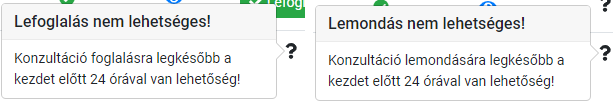
\includegraphics[width=10cm]{kepek/screenshots/hallgato_konzultacio_foglal_lemond_hibak.png}
		\caption{Foglaláskor és lemondáskor megjelenő hibaüzenetek}
		\label{fig:hallgato_konzultacio_foglal_lemond_hibak}
	\end{figure}
	
	\subsection{Mérföldkövek}
	A \emph{,,Mérföldkövek''} menüpont alatt tekinthető meg az összes a hallgató szakdolgozatához tartozó mérföldkő. Amennyiben a hallgatóhoz még nincsen szakdolgozat társítva, vagy nincsen a szakdolgozatához kapcsolódó mérföldkő, úgy a \emph{,,A keresett feltételekkel nem található mérföldkő!''} hibaüzenet jelenik meg az oldalon (\ref{fig:hallgato_merfoldko_nincs}.~ábra).
	
	\begin{figure}[!h]
		\centering
		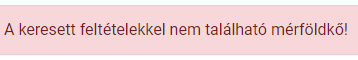
\includegraphics[width=8cm]{kepek/screenshots/hallgato_merfoldko_nincs.png}
		\caption{Hibaüzenet, ha a hallgatónak nincs szakdolgozata, vagy mérföldköve}
		\label{fig:hallgato_merfoldko_nincs}
	\end{figure}
	
	A kilistázott mérföldkövek között a táblázat fölötti szűrési lehetőségek használatával lehet keresni név, és állapot alapján, illetve lehetőség van határidő szerint növekvő és csökkenő sorrendbe rendezve megtekinteni azokat (\ref{fig:hallgato_merfoldko_lista}.~ábra). A még nem lejárt feladatok határideje piros, vastagított betűvel vannak jelezve. A műveletek oszlopban található kék ikonnal megnyitható a mérföldkő adatlapja (\ref{fig:hallgato_merfoldko_adatlap}.~ábra), ahol a hallgató elolvashatja a feladat leírását, a feladathoz tartozó címkéket, és lehetősége van a feladathoz megjegyzést hozzáfűzni, esetlegesen a megjegyzéshez csatolmányként fájlokat küldeni.
	
	\begin{figure}[!h]
		\centering
		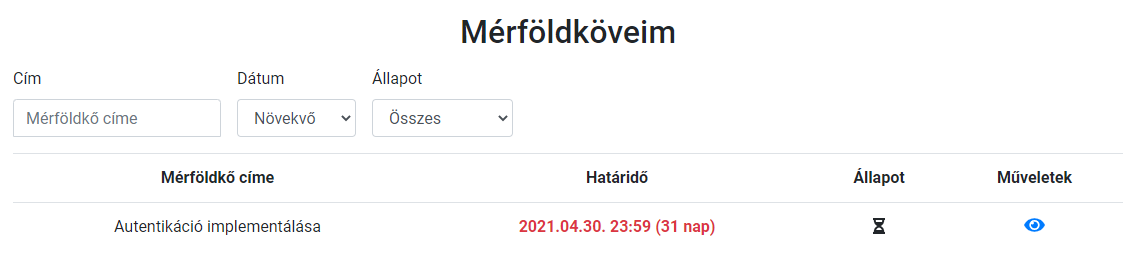
\includegraphics[width=12cm]{kepek/screenshots/hallgato_merfoldko_lista.png}
		\caption{Mérföldkövek listája}
		\label{fig:hallgato_merfoldko_lista}
	\end{figure}
	
	\begin{figure}[!h]
		\centering
		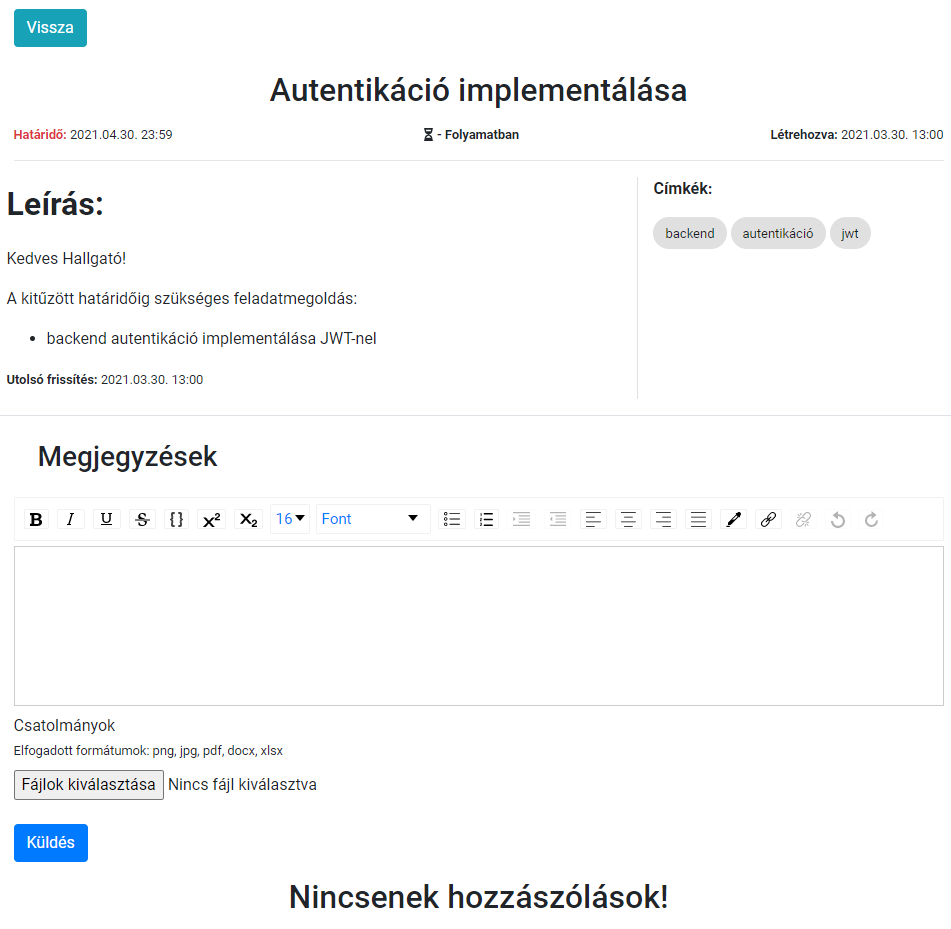
\includegraphics[width=11cm]{kepek/screenshots/hallgato_merfoldko_adatlap.png}
		\caption{Mérföldkő adatlapja}
		\label{fig:hallgato_merfoldko_adatlap}
	\end{figure}
	
	\chapter{Összefoglalás}
	Szakdolgozatomban a webes platform és az ott használatos protokollok, architektúrák áttekintése után megvizsgáltam és összehasonlítottam a piacon manapság legnépszerűbb webes technológiákat. Az alkalmazás specifikációjának ismertetése után pedig bemutattam a fejlesztett alkalmazás használatát.
	
	A jövőre vonatkozóan többek között az alábbi terveket fogalmaztam meg: 
	\begin{itemize}
		\item az ügyintézők által kezelhető ügyek bővítése
		\item egy email visszajelző rendszer kiépítése, amely mérföldkövek vagy konzultációs időpontokkal kapcsolatos változások esetén üzenetet küldene az érintett oktató és hallgató számára
		\item a konzultációs időpontok jobb átláthatósága érdekében egy naptár nézetet létrehozni, Google Naptár vagy akár telefonos naptárba való exportálás lehetőségével
		\item az oldal többnyelvűsítése, hogy azt külföldi személyek is használhassák.
	\end{itemize}
	Úgy gondolom, hogy a szakdolgozat elején megfogalmazott célokat sikerült elérnem. Reményeim szerint sikerült egy olyan webes alkalmazást készítenem, amelynek tényleg hasznát vehetik az oktatók és hallgatók egyaránt, és hatékonyabbá teheti a munkát és az ahhoz kapcsolódó visszajelzést.
\begin{thebibliography}{10}
\bibitem{howthewebworks} 
How the Web works (2021.02.08.)
\\\url{https://developer.mozilla.org/en-US/docs/Learn/Getting\_started\_with\_the\_web/How\_the\_Web\_works}
\bibitem{internetprotocols}
Internet Protocols (2021.02.08.)
\\\url{https://www.tutorialspoint.com/internet\_technologies/internet\_protocols.htm}
\bibitem{sshprotocol} 
SSH Protocol – Secure Remote Login and File Transfer (2021.02.08.)
\\\url{https://www.ssh.com/ssh/protocol/}
\bibitem{httpdocs} 
HTTP (2021.02.08.)
\\\url{https://developer.mozilla.org/en-US/docs/Web/HTTP}
\bibitem{clientserver_overview} 
Client-Server Overview (2021.02.08.)
\\\url{https://developer.mozilla.org/en-US/docs/Learn/Server-side/First\_steps/Client-Server\_overview}
\bibitem{tierarchitecture}
Three tier architecture (2021.02.08.)
\\\url{https://www.ques10.com/p/29000/explain-three-tier-architecture-with-advantages-di/}
\bibitem{jquery}
JQuery (2021.02.15.)
\\\url{https://jquery.com/}
\bibitem{stackoverflow_survey}
Stack Overflow Developer Survey 2020 (2021.02.10.)
\\\url{https://insights.stackoverflow.com/survey/2020\#most-popular-technologies}
\bibitem{stackoverflow_trends}
Stackoverflow Trends (2021.02.10.)
\\\url{https://insights.stackoverflow.com/trends}
\bibitem{octoverse}
The State of the Octoverse (2021.02.10.)
\\\url{https://octoverse.github.com/}
\bibitem{vuecomparison}
Comparison with Other Frameworks (2021.02.25.)
\\\url{https://vuejs.org/v2/guide/comparison.html}
\bibitem{vuedocs}
Vue dokumentáció (2021.04.15.)
\\\url{https://v3.vuejs.org/guide/}
\bibitem{angulardocs}
Introduction to the Angular Docs (2021.03.01.)
\\\url{https://angular.io/docs}
\bibitem{react}
React (2021.02.10.)
\\\url{https://reactjs.org/}
\bibitem{redux}
Redux (2021.04.18.)
\\\url{https://redux.js.org/introduction/getting-started}
\bibitem{expressnodeintro}
Express/Node introduction (2021.04.08.)
\\\url{https://developer.mozilla.org/en-US/docs/Learn/Server-side/Express\_Nodejs/Introduction}
\bibitem{expressdocs}
Express.js (2021.04.08.)
\\\url{https://expressjs.com/}
\bibitem{nestdocs}
NestJS Documentation (2021.04.08.)
\\\url{https://docs.nestjs.com/}
\bibitem{relationalvsnon-relational}
Relational vs. non-relational databases (2021.03.04.)
\\\url{https://www.pluralsight.com/blog/software-development/relational-vs-non-relational-databases}
\bibitem{ibm_sqlvsnosql}
SQL vs. NoSQL Databases: What's the Difference? (2021.03.04.)
\\\url{https://www.ibm.com/cloud/blog/sql-vs-nosql}
\bibitem{mongo_typeofnosqldbs}
Understanding the Different Types of NoSQL Databases (2021.03.04.)
\\\url{https://www.mongodb.com/scale/types-of-nosql-databases}
\bibitem{aws_graphdb}
What Is a Graph Database? (2021.03.04.)
\\\url{https://aws.amazon.com/nosql/graph/}
\bibitem{mongodb_json_bson}
JSON and BSON | MongoDB (2021.03.04.)
\\\url{https://www.mongodb.com/json-and-bson}
\end{thebibliography}
\includepdf[pages=1,pagecommand={}]{nyilatkozat.pdf}
\end{document}